% !TeX root = main.tex
\chapter{Експериментальні дослідження інформаційної технології виявлення аномальних кодів у фото- та відеооб’єктах веб-ресурсів}
\label{chap:experiments}

\section{Мета, завдання та загальна організація експериментальних досліджень}

У розділах 2 і 3 сформовано модель мультимодального представлення прихованої загрози, метод спектрально-зорового та структурного аналізу, метод поведінкового узгодження ознак різного походження та п’ятиетапну інформаційну технологію. Експериментальне дослідження має встановити, які властивості цих результатів підтверджуються вимірюваннями, а які залишаються формалізованими положеннями. Таке розмежування потрібне, оскільки наявність повної архітектурної схеми ще не доводить працездатності кожного її складника, а високий показник на одному наборі не підтверджує переносимості рішення на нові мультимедійні об’єкти.

Метою експериментальних досліджень є оцінювання здатності детермінованих структурних і спектрально-зорових ознак розрізняти мультимедійні об’єкти без контрольованої зміни та об’єкти із заданими структурними або статистичними відхиленнями, а також визначення меж, у яких результати прототипної конфігурації можна використовувати для обґрунтування інформаційної технології. Мета охоплює не лише обчислення показників, а й перевірку походження даних, способу їх поділу, незмінності параметрів під час оцінювання та відповідності висновку фактично виконаним операціям.

Дослідницьке припущення полягає в тому, що спільний статичний опис $H$, утворений зі структурних $Z_s$ і спектрально-зорових $Z_v$ ознак, забезпечує повніше розрізнення контрольованих змін, ніж використання лише спектрально-зорового представлення. Перевірка цього припущення не поширюється автоматично на повне інтегроване представлення $Z$, оскільки для нього потрібні причинно пов’язані події $X_b$, подієво-поведінкові ознаки $Z_b$ та ознака їх доступності $m_b$. У проведеному контрольованому експерименті такі журнали не формувалися, тому оцінюється саме статична частина першого методу.

Послідовне виявлення обмежень зумовило шість окремих експериментальних серій і додаткове ресурсне вимірювання. Ретроспективний прогін на $110$ об’єктах дав агреговані орієнтири. У внутрішньому контрольованому циклі сформовано $200$ груп походження і $400$ PNG- та MP4-об’єктів, визначено параметри трьох статичних конфігурацій та виконано одноразове оцінювання на недоторканій перевірній частині. Цей цикл показав перевагу спільного статичного опису над ізольованими спектрально-зоровими ознаками, але через синтетичне походження даних не відповідав на питання зовнішньої переносимості.

Наступні серії послідовно перевіряли саме це обмеження. Перша зовнішня перевірка на природних відеозаписах не відтворила внутрішньої переваги спільного опису над структурною конфігурацією та виявила нестійкість спектрально-зорових оцінок. Поетапна підтверджувальна серія показала, що додаткова вимога підтвердження усуває частину хибнопозитивних рішень, але збільшує кількість пропусків. Після цього великомасштабну перевірку розширено від $2000$ MP4 до $10\,000$ фізичних об’єктів п’яти форматів, утворених із $500$ базових відеофрагментів. На цих даних сформовано скорочений навчуваний шлюз узгодження вихідних оцінок першого методу, а його незмінні параметри перевірено в окремій шостій серії на $2000$ об’єктах із чотирьох нових пристроїв. Ресурсне вимірювання в п’яти незалежних процесних запусках доповнило показники рішень 95-м процентилем наскрізного часу та найбільшим обсягом фізичної пам’яті процесу. Отже, процес дослідження охопив не лише підтвердження початкового припущення, а й його послідовне звуження, перевірку форматного перенесення та встановлення ціни одержаного результату в обчислювальних ресурсах.

Для досягнення поставленої мети розв’язано такі завдання:

\begin{enumerate}
\item сформовано контрольований набір із груповим поділом, який унеможливлює одночасне потрапляння об’єктів спільного походження до частин навчання й перевірки;
\item визначено структурну, спектрально-зорову та спільну статичну конфігурації, а також єдиний порядок їх навчання, налаштування й оцінювання;
\item обчислено показники рішень на недоторканій перевірній частині, оцінено їх невизначеність і виконано парне зіставлення конфігурацій;
\item досліджено залежність результатів від формату, виду контрольованої зміни та складу ознак;
\item перевірено перенесення незмінних параметрів на природні відеозаписи з пристроїв, які не використовувалися для навчання й добору порога;
\item досліджено, чи зменшує правило підтвердження спектрального спрацювання частку хибнопозитивних рішень без неприйнятного зменшення повноти;
\item перевірено форматне перенесення незмінних параметрів на PNG, JPEG, WebP, MP4 і WebM та стабільність установлених закономірностей на $500$ базових фрагментах без прирівнювання похідних об’єктів до незалежних джерел;
\item сформовано скорочений навчуваний шлюз узгодження статичних оцінок і виконано його незалежну перевірку на об’єктах із чотирьох нових пристроїв без повторного навчання та добору порога;
\item виміряно 95-й процентиль наскрізного часу й найбільший обсяг фізичної пам’яті процесу для порівнюваних конфігурацій у п’яти незалежних процесних запусках;
\item обчислено розвідувальний інтегральний показник ефективності, що поєднує достовірність виявлення, часові витрати, пам’ять і стійкість результату між форматами, та окремо застосовано обов’язковий форматний допуск;
\item перевірено арифметичну узгодженість збережених агрегатів попереднього прогону й установлено межі їх предметного тлумачення.
\end{enumerate}

Призначення шести серій і допустиму силу висновків узагальнено в табл.~\ref{tab:ch4_research_program}. Кожна наступна серія відповідала на обмеження, виявлене попередньою. Через відмінність джерел, співвідношення класів і способів формування об’єктів їхні показники не об’єднуються в одну вибірку й не трактуються як послідовне підвищення якості.

\begin{table}[htbp]
\caption{Організація експериментальних досліджень}
\label{tab:ch4_research_program}
\centering
\scriptsize
\begin{tabularx}{\textwidth}{p{0.17\textwidth}p{0.22\textwidth}Y Y}
\toprule
Цикл & Експериментальний матеріал & Призначення & Допустимий висновок \\
\midrule
Ретроспективний & Агрегований опис $110$ об’єктів, матриця рішень, компонентні й часові підсумки & Перевірка арифметики та внутрішніх залежностей попереднього прогону & Узгодженість повідомлених агрегатів без висновку про незалежне відтворення чи узагальнення \\
Внутрішній контрольований & $200$ первинних груп, $400$ об’єктів, поділ $60:20:20$, пооб’єктні ознаки й рішення & Навчання контрольних моделей і перевірка статичного опису $H$ & Кількісна оцінка детермінованих ознак у межах синтетичних PNG і MP4 \\
Перша зовнішня перевірка & $14$ природних MP4, $8$ груп ``пристрій--сцена'', $56$ похідних об’єктів & Перевірка незмінних параметрів на новому походженні & Оцінка перенесення на чотири зовнішні пристрої без перенавчання \\
Поетапна підтверджувальна & $8$ нових MP4, $4$ групи, $32$ парні об’єкти & Перевірка першого методу, доступної правилової ознаки та правила підтвердження & Установлення зміни співвідношення між хибнопозитивними рішеннями й пропусками \\
Великомасштабна багатоформатна & $8$ джерел, $500$ базових фрагментів, $10\,000$ похідних об’єктів п’яти форматів & Перевірка форматного перенесення, порівняння конфігурацій і формування навчуваного шлюзу & Уточнення повторюваності в межах двох пристроїв без висновку про $10\,000$ незалежних джерел \\
Незалежна підтверджувальна & $8$ нових джерел із $4$ пристроїв, $100$ базових фрагментів, $2000$ об’єктів & Одноразова перевірка зафіксованого навчуваного шлюзу & Оцінка зміни типів помилок і перенесення на нові пристрої без повторного навчання \\
\bottomrule
\end{tabularx}
\end{table}

Загальну організацію дослідження показано на рис.~\ref{fig:experimental_setup}. Послідовність від попереднього прогону до незалежної багатоформатної перевірки відображає не накопичення дедалі вищих показників, а перевірку початкового результату за жорсткіших умов. Негативний зовнішній результат спектрально-зорової гілки збережено як самостійний науковий результат, оскільки саме він визначив подальшу процедуру.

\begin{figure}[htbp]
\centering
\begin{tikzpicture}[x=1cm,y=1cm]
\node[dissertation block,text width=3.30cm,minimum height=1.15cm] (preliminary) at (-4.5,1.5)
  {Попередній прогін};
\node[dissertation block,text width=3.30cm,minimum height=1.15cm] (internal) at (0,1.5)
  {Внутрішній цикл};
\node[dissertation block,text width=3.30cm,minimum height=1.15cm] (external) at (4.5,1.5)
  {Перша зовнішня\\перевірка};

\node[dissertation block,text width=3.55cm,minimum height=1.15cm] (confirmatory) at (4.5,-1.5)
  {Поетапна\\перевірка};
\node[dissertation block,text width=3.30cm,minimum height=1.15cm] (large) at (0,-1.5)
  {Багатоформатна\\серія};
\node[dissertation block,text width=3.30cm,minimum height=1.15cm] (independent) at (-4.5,-1.5)
  {Відкладена зовнішня\\перевірка};

\draw[dissertation arrow] (preliminary.east) -- (internal.west);
\draw[dissertation arrow] (internal.east) -- (external.west);
\draw[dissertation arrow] (external.south) -- (confirmatory.north);
\draw[dissertation arrow] (confirmatory.west) -- (large.east);
\draw[dissertation arrow] (large.west) -- (independent.east);
\end{tikzpicture}
\caption{Послідовність експериментальних серій дослідження}
\label{fig:experimental_setup}
\end{figure}


Об’єктом кількісної перевірки є детермінована частина методу спектрально-зорового та структурного аналізу, яка формує $Z_s$, $Z_v$ і спільний статичний опис $H$, а також скорочений навчуваний шлюз, що узгоджує три вихідні оцінки першого методу, дві їхні розбіжності та ознаку формату. Цей шлюз перевіряє можливість навчуваного узгодження вже сформованих статичних свідчень, але не замінює повного методу поведінкового узгодження. Причинно пов’язані журнали $X_b$, повне представлення $Z_b$, кодувальник послідовностей і перехресне зіставлення у проведених серіях не формувалися.

Таке обмеження не применшує одержаних результатів, а визначає їх точний зміст. Висновок про статичний опис не можна переносити на всю мультимодальну технологію, однак послідовність внутрішньої й зовнішніх серій дає змогу перевірити, чи зберігається спостережувана доповнювальність ознак після зміни походження даних. Для виконання поставлених завдань використано кілька неперетинних наборів, які відрізняються складом первинних записів і допустимою силою висновку.

\section{Формування експериментального набору даних і середовища досліджень}

Основний набір сформовано спеціально для перевірки детермінованих складників першого методу. Вихідною одиницею є первинна група, яка поєднує об’єкт без контрольованої зміни та похідний від нього об’єкт із заданим відхиленням. Завдяки цьому рішення для двох версій можна зіставляти, не втрачаючи відомостей про спільне походження. Загалом утворено $200$ первинних груп: $160$ груп PNG і $40$ груп MP4. Кожна група містила два об’єкти, тому повний обсяг набору становив $400$.

Базові зображення сформовано з гармонічних складників, шумових реалізацій і геометричних фігур. Розмір PNG дорівнював $256\times256$ пікселів. Відео мало розмір кадру $160\times120$ пікселів, складалося з $12$ кадрів і кодувалося з частотою $12$ кадрів за секунду. Положення фігур у послідовності змінювалося, тому часові ознаки відео не зводилися до повторення одного нерухомого кадру. Синтетичне походження забезпечило керованість змін, але водночас обмежило переносимість результату на природні фото- й відеодані.

Поділ виконано на рівні первинних груп у співвідношенні $60:20:20$. До навчальної частини ввійшло $120$ груп і $240$ об’єктів, до налаштувальної --- $40$ груп і $80$ об’єктів, до перевірної --- $40$ груп і $80$ об’єктів. Спочатку групи розподілено зі збереженням співвідношення форматів і видів змін, і лише після цього створено похідні об’єкти. Отже, дві версії одного базового вмісту завжди належали до тієї самої частини. Склад набору наведено в табл.~\ref{tab:ch4_ind_svs_dataset}.

\begin{table}[htbp]
\caption{Склад групово відокремленого експериментального набору}
\label{tab:ch4_ind_svs_dataset}
\centering
\small
\begin{tabular}{lrrrrrr}
\toprule
Формат & Групи & Без зміни & Зі зміною & Навчальна & Налаштувальна & Перевірна \\
\midrule
PNG & 160 & 160 & 160 & 192 & 64 & 64 \\
MP4 & 40 & 40 & 40 & 48 & 16 & 16 \\
\midrule
Разом & 200 & 200 & 200 & 240 & 80 & 80 \\
\bottomrule
\end{tabular}
\end{table}

Груповий поділ усуває один із головних чинників завищення показників. Якби похідні того самого вмісту опинилися одночасно в навчальній і перевірній частинах, класифікаційна модель могла б використати властивості джерела замість ознак контрольованої зміни. Поділ за назвою готового об’єкта цього не гарантує, тому належність до первинної групи фіксувалася окремим ідентифікатором.

Для представлення різних механізмів утворено чотири види контрольованих змін, наведені в табл.~\ref{tab:ch4_ind_svs_changes}. Кожному виду відповідало $50$ первинних груп у повному наборі, з них $30$ груп належали до навчальної, $10$ --- до налаштувальної і $10$ --- до перевірної частини. Розподіл забезпечив однакову кількість перевірних позитивних об’єктів для кожного виду, що дало змогу встановити, який саме механізм визначає пропуски спільної конфігурації.

\begin{table}[htbp]
\caption{Види контрольовано внесених змін у групово відокремленому експерименті}
\label{tab:ch4_ind_svs_changes}
\centering
\scriptsize
\begin{tabularx}{\textwidth}{p{0.20\textwidth}Y Y}
\toprule
Вид зміни & PNG & MP4 \\
\midrule
Хвостове додавання & Додавання $2048$ байтів після логічного завершення структури & Додавання $4096$ байтів після наявного контейнера \\
Допоміжний блок користувацького типу & Додавання перед IEND блока обсягом $2048$ байтів із коректною контрольною сумою & Додавання контейнерного блока \texttt{free} з навантаженням $4096$ байтів \\
Спектральна зміна & Шахове відхилення синього каналу на $\pm2$ для $18$~\% пікселів і зміна молодшого біта для $12$~\% значень & Покадрове шахове відхилення синього каналу на $\pm(2\ldots4)$ для $16$~\% пікселів \\
Поєднана зміна & Спектральна зміна разом із хвостовим додаванням $2048$ байтів & Спектральна зміна разом із хвостовим додаванням $4096$ байтів \\
\bottomrule
\end{tabularx}
\end{table}

Перші два види утворюють виразне структурне свідчення, яке можна виявити під час розбору контейнера. Спектральна зміна не порушує формальної будови й має проявлятися в декодованому представленні. Поєднана зміна одночасно надає свідчення двом статичним гілкам. Такий склад потрібний для порівняння ізольованих і спільної конфігурацій, але не охоплює всіх способів прихованого розміщення даних.

Для кожного об’єкта збережено його ідентифікатор, ідентифікатор первинної групи, частину поділу, формат, еталонну мітку, вид зміни, розмір, початкове значення генератора випадкових чисел і контрольну суму SHA-256. Окремі машинозчитувані записи містять виділені ознаки, неперервні оцінки трьох конфігурацій, пороги, рішення та часові вимірювання. Повторна автоматична перевірка підтвердила $400$ записів реєстру, $200$ груп, успішне декодування $320$ PNG і $80$ MP4 та $240$ перевірних прогнозів, тобто по $80$ для кожної конфігурації.

Структурне представлення містило дев’ять ознак: результати перевірки сигнатури, синтаксичного розбору та цілісності, відношення хвостових байтів і допоміжного навантаження до розміру об’єкта, частку невідомих елементів, масштабовану кількість структурних елементів, невідповідність розміру та ознаку відеоконтексту. Для PNG аналізували послідовність блоків, контрольні суми, завершальну структуру й додаткові байти. Для MP4 перевіряли типи й межі контейнерних блоків, блоки \texttt{free} та залишок після останнього коректного блока.

Спектрально-зорове представлення містило шістнадцять ознак. До них належали ентропійні, лапласіанні, хвилькові й косинусні характеристики, частота переходів молодших бітів, ознаки синього каналу, міжканальний залишок і часові відмінності між кадрами. Для PNG часові характеристики дорівнювали нулю, оскільки об’єкт містив одне зображення. Спільний статичний опис $H$ містив $24$ ознаки: дев’ять структурних і п’ятнадцять додаткових спектрально-зорових, оскільки ознаку відеоконтексту не дублювали. Призначення трьох конфігурацій узагальнено в табл.~\ref{tab:ch4_feature_configs}.

\begin{table}[htbp]
\caption{Конфігурації ознак у групово відокремленому експерименті}
\label{tab:ch4_feature_configs}
\centering
\small
\begin{tabularx}{\textwidth}{p{0.23\textwidth}p{0.13\textwidth}Y Y}
\toprule
Конфігурація & Кількість & Основні групи ознак & Призначення \\
\midrule
Структурна $Z_s$ & 9 & Сигнатура, синтаксис, цілісність, хвостові області, допоміжні блоки, розміри & Перевірка контейнерного рівня без використання декодованого вмісту \\
Спектрально-зорова $Z_v$ & 16 & Ентропія, залишки, перетворення Гаара, дискретне косинусне перетворення, бітові й часові характеристики & Перевірка декодованого подання без структурних правил контейнера \\
Спільний статичний опис $H$ & 24 & Узгоджений вектор $Z_s$ і $Z_v$ без дублювання відеоконтексту & Оцінювання доповнювальності двох статичних джерел ознак \\
\bottomrule
\end{tabularx}
\end{table}

Фінальний запуск виконано з початковим значенням генератора $20260717$ у Windows~11 із Python~3.13.3, NumPy~2.3.0 та OpenCV~4.10.0; декодування MP4 забезпечувала вбудована підтримка FFmpeg. Початкове значення $20260716$, використане під час попереднього налагодження, до підсумкового оцінювання не входило. У паспорті фінального запуску не зафіксовано апаратну конфігурацію, тому часові значення характеризують саме цю програмну реалізацію й не є апаратно незалежною оцінкою.

Після внутрішнього циклу параметри трьох контрольних моделей і пороги зафіксовано у файлі параметрів. Його контрольна сума однакова в усіх зовнішніх серіях, що підтверджує відсутність перенавчання й добору порога за новими даними. Зовнішні набори утворено з природних відеозаписів VISION, одержаних різними портативними пристроями в приміщенні та поза ним. Використано як первинні записи, так і версії після опрацювання відеоплатформою.

Перша зовнішня вибірка містила $14$ MP4 із чотирьох пристроїв: вісім первинних і шість опрацьованих платформою записів. Їх об’єднано у вісім груп ``пристрій--сцена'', щоб пов’язані варіанти одного походження залишалися однією одиницею оцінювання невизначеності. З кожного джерела детерміновано відібрано $12$ послідовних кадрів із ділянки на рівні $20$~\% тривалості. Співвідношення сторін збережено доповненням полів до $320\times240$ пікселів.

Для кожного відібраного фрагмента сформовано чотири умови: без контрольованої зміни, зі структурним блоком, зі спектральною зміною та з поєднанням двох змін. Отже, перша зовнішня серія охопила $56$ похідних об’єктів. Структурне втручання полягало в додаванні коректного термінального блока \texttt{free} з $32768$ детермінованими байтами. Спектральне втручання відтворювало малоамплітудну зміну синього каналу для $16$~\% пікселів кожного кадру. Оригінали не змінювалися; усі операції виконувалися лише над зареєстрованими копіями.

Підтверджувальну серію сформовано з восьми нових MP4 двох інших пристроїв, які утворили чотири групи ``пристрій--сцена'' та $32$ похідні об’єкти. Її призначенням було поетапне порівняння стану до застосування методів, після першого методу, після доступної правилової частини другого методу та після введення правила підтвердження спектрального спрацювання. Параметри й порядок зіставлення зафіксовано до відкриття результатів цієї серії.

Великомасштабний набір сформовано з восьми природних MP4 двох інших пристроїв. Із неперетинних часових вікон утворено $500$ базових 12-кадрових фрагментів. Кожний фрагмент подано у форматах PNG, JPEG, WebP, MP4 і WebM та в чотирьох умовах: контрольній, структурній, спектральній і поєднаній. Отже, один базовий фрагмент породжував $20$ фізичних об’єктів, а повний обсяг становив $10\,000$, по $2000$ кожного формату. PNG і MP4 належали до початкової області моделей першого методу; JPEG, WebP і WebM оцінювалися як перенесення незмінних параметрів без повторного навчання чи добору порога.

На цьому самому наборі сформовано скорочений навчуваний шлюз узгодження. Його вхід містив структурну, спектрально-зорову та спільну оцінки першого методу, дві різниці між ними й п’ять ознак формату. Мережа мала $10$ входів, $6$ прихованих вузлів, один вихід і $73$ параметри. Об’єкти одного джерела не розподілялися між етапами: $2500$ об’єктів із записів одного пристрою в приміщенні використано для навчання, $2500$ з іншої сцени того самого пристрою --- для визначення порога, а $5000$ об’єктів другого пристрою --- для внутрішньої перевірки. Тому результати шлюзу на цих $10\,000$ об’єктах характеризують етап розроблення, а не незалежне підтвердження.

Для незалежного підтвердження використано вісім інших природних записів із чотирьох нових пристроїв. Із них утворено $100$ базових фрагментів і $2000$ похідних об’єктів за тією самою схемою п’яти форматів і чотирьох умов. Параметри шлюзу та поріг зафіксовано до виділення ознак цієї вибірки. Контрольні суми й адреси первинних записів не перетиналися з попередніми зовнішніми наборами, тому цей цикл використано для перевірки перенесення навчуваного узгодження.

Ресурсне вимірювання проведено на стратифікованій підмножині великомасштабного набору. Із кожного з восьми вихідних записів відібрано по чотири базові фрагменти, яким однозначно призначено чотири умови; кожний фрагмент подано в усіх п’яти форматах. У результаті загальні конфігурації опрацьовували $160$ фізичних об’єктів, а конфігурації з доступною відеоознакою --- $64$ MP4- і WebM-об’єкти. Вимірювання повторено в п’яти окремих процесах за одного робочого потоку й одного потоку засобу комп’ютерного зору. Холодний запуск процесу не включали до пооб’єктного часу. Апаратний паспорт не зафіксовано, тому одержані значення характеризують записане програмне середовище, але не є апаратно незалежними.

Склад і призначення зовнішніх серій зіставлено в табл.~\ref{tab:ch4_external_sets}. Кількість похідних об’єктів у цій таблиці не є кількістю незалежних джерел: найбільша серія містить лише вісім вихідних записів, а незалежна підтверджувальна --- також вісім.

\begin{table}[htbp]
\caption{Склад зовнішніх експериментальних серій на природних відеозаписах}
\label{tab:ch4_external_sets}
\centering
\scriptsize
\begin{tabularx}{\textwidth}{p{0.20\textwidth}rrr p{0.19\textwidth}Y}
\toprule
Серія & Пристрої & Джерела & Базові одиниці & Похідні об’єкти & Призначення \\
\midrule
Перша зовнішня & 4 & 14 & 8 груп & 56 MP4 & Перевірка незмінних моделей і порогів на новому походженні \\
Поетапна підтверджувальна & 2 & 8 & 4 групи & 32 MP4 & Перевірка правила підтвердження \\
Багатоформатна & 2 & 8 & 500 фрагментів & $10\,000$ об’єктів п’яти форматів & Перенесення першого методу, розроблення шлюзу та оцінювання стійкості \\
Незалежна підтверджувальна & 4 & 8 & 100 фрагментів & $2000$ об’єктів п’яти форматів & Перевірка зафіксованого шлюзу на нових пристроях \\
\bottomrule
\end{tabularx}
\end{table}

Для кожної зовнішньої серії збережено адреси й контрольні суми первинних записів, відомості про пристрій, варіант і сцену, параметри формування похідних, ознаки, неперервні оцінки, рішення та опис програмного середовища. Автоматична перевірка підтвердила очікувані $10\,000$ і $2000$ фізичних об’єктів, повноту форматно-сценарних блоків, відсутність накладання часових вікон, збіг контрольних сум і відсутність перетину первинних записів між зовнішніми наборами. Це не збільшує кількість незалежних пристроїв, але дає змогу відокремити розроблення від підтвердження.

Ретроспективний набір мав інше походження. За збереженим описом він містив $110$ об’єктів: $100$ PNG і $10$ MP4. До контрольного класу належали $50$ PNG і $5$ MP4, а до класу з навмисно внесеними відхиленнями --- така сама кількість. Структуру форматів і класів показано на рис.~\ref{fig:dataset_structure}.

\begin{figure}[htbp]
\centering
\begin{tikzpicture}[x=1cm,y=1cm]
\node[dissertation block,text width=3.70cm] (all) at (0,3.2)
  {Контрольний набір\\110 об’єктів};

\node[dissertation block,text width=3.15cm] (png) at (-3.3,1.2)
  {PNG\\100 об’єктів};
\node[dissertation block,text width=3.15cm] (mp4) at (3.3,1.2)
  {MP4\\10 об’єктів};

\node[dissertation block,text width=2.75cm] (pngctrl) at (-5.1,-1.4)
  {Контрольні PNG\\50};
\node[dissertation block,text width=2.75cm] (pngmod) at (-1.7,-1.4)
  {Змінені PNG\\50};
\node[dissertation block,text width=2.75cm] (mp4ctrl) at (1.7,-1.4)
  {Контрольні MP4\\5};
\node[dissertation block,text width=2.95cm] (mp4tail) at (5.1,-1.4)
  {MP4 із хвостовим\\маркером, 5};

% Розподільні шини утворюють лише прямокутні траєкторії.
\coordinate (formatbus) at (0,2.25);
\draw[thick] (all.south) -- (formatbus);
\draw[thick] (-3.3,2.25) -- (3.3,2.25);
\draw[dissertation arrow] (-3.3,2.25) -- (png.north);
\draw[dissertation arrow] (3.3,2.25) -- (mp4.north);

\coordinate (pngbus) at (-3.3,-0.05);
\draw[thick] (png.south) -- (pngbus);
\draw[thick] (-5.1,-0.05) -- (-1.7,-0.05);
\draw[dissertation arrow] (-5.1,-0.05) -- (pngctrl.north);
\draw[dissertation arrow] (-1.7,-0.05) -- (pngmod.north);

\coordinate (mpfourbus) at (3.3,-0.05);
\draw[thick] (mp4.south) -- (mpfourbus);
\draw[thick] (1.7,-0.05) -- (5.1,-0.05);
\draw[dissertation arrow] (1.7,-0.05) -- (mp4ctrl.north);
\draw[dissertation arrow] (5.1,-0.05) -- (mp4tail.north);
\end{tikzpicture}
\caption{Форматний і класовий склад контрольного набору за контрольним описом}
\label{fig:dataset_structure}
\end{figure}


Серед змінених PNG було по $10$ об’єктів із послідовною та випадковою зміною молодших бітів, хвильковим внесенням, хвостовою областю після IEND і текстовим сценарним фрагментом після завершальної структури. П’ять змінених MP4 містили хвостовий маркер після контейнера. Позитивна мітка в усіх серіях позначає контрольовано внесене відхилення, а не доведене виконання аномального коду або небезпечну дію веб-системи.

Для попереднього прогону повідомлено апаратну конфігурацію AMD Ryzen~7~5700X із $32$~ГБ оперативної пам’яті та послідовний режим на центральному процесорі. Однак первинного журналу запуску, реєстру походження, контрольних сум об’єктів і програмного коду не збережено. Крім того, параметри налаштовували й оцінювали на тому самому наборі. Отже, цей набір придатний для арифметичної перевірки зведених значень, але не для незалежної оцінки здатності до узагальнення.

Оскільки набори сформовано за різними протоколами, їхні числові результати не об’єднуються і не трактуються як зміна якості одного випробування. Внутрішній цикл відповідає на питання про статичний опис $H$ у контрольованих синтетичних умовах; перші дві зовнішні серії перевіряють перенесення на природні MP4; багатоформатна серія встановлює форматну залежність і забезпечує дані для розроблення шлюзу; незалежна підтверджувальна серія перевіряє його незмінну конфігурацію; ретроспективний матеріал характеризує внутрішню узгодженість раніше зафіксованого прогону.

\section{Методика проведення експериментів і метрики оцінювання}

\subsection{Послідовність основного експерименту}

Методику основного циклу побудовано так, щоб відокремити формування даних, визначення параметрів і підсумкове оцінювання. Кожний етап усуває конкретне джерело викривлення: груповий поділ запобігає витоку відомостей про спільне походження, окрема налаштувальна частина не допускає добору порога за перевірними мітками, а одноразове оцінювання зберігає незалежність підсумкового результату.

Послідовність виконання основного експерименту була такою:

\begin{enumerate}
\item \textit{Розподіл первинних груп.} До створення похідних $200$ груп розподілено між навчальною, налаштувальною та перевірною частинами. Співвідношення форматів і видів змін збережено в кожній частині.

\item \textit{Формування пар об’єктів.} Для кожної групи створено версію без контрольованої зміни та одну змінену версію. Еталонну мітку зберігали в реєстрі підготовки; модуль виділення ознак не використовував її як вхід.

\item \textit{Виділення ознак.} Для кожного об’єкта окремо сформовано $Z_s$, $Z_v$ і спільний статичний опис $H$. Це дало змогу порівнювати конфігурації на тих самих об’єктах і за однакових умов декодування.

\item \textit{Навчання контрольних моделей.} Для трьох конфігурацій використано однакову стандартизовану логістичну регресію з $L_2$-регуляризацією $0{,}05$. Середні значення, масштаби й коефіцієнти визначено лише за $240$ навчальними об’єктами. Класифікаційна модель виконувала роль контрольного засобу оцінювання ознак і не вводилася як новий складник методу.

\item \textit{Визначення порогів.} Порогові значення вибрано лише за $80$ налаштувальними об’єктами за найбільшою збалансованою часткою правильних рішень. Для структурної, спектрально-зорової та спільної конфігурацій вони становили відповідно $0{,}328738$, $0{,}481738$ і $0{,}456468$. Після цього коефіцієнти й пороги залишалися незмінними.

\item \textit{Одноразова перевірка.} Підсумкові прогнози одержано на $80$ об’єктах із $40$ первинних груп, які не використовувалися для навчання, приведення ознак до спільного масштабу або визначення порога. Лише після фіксації прогнозів їх зіставлено з еталонними мітками.

\item \textit{Оцінювання невизначеності й парних відмінностей.} Для довірчих інтервалів виконано $2000$ повторних групових вибирань із поверненням. В одному повторенні вибирали $40$ первинних груп і включали обидва пов’язані об’єкти кожної групи. Парні розбіжності правильності додатково оцінено точним двобічним критерієм Мак-Немара на тих самих $80$ об’єктах.

\item \textit{Вимірювання часу та перевірка артефактів.} Час структурного й спектрально-зорового оброблення фіксували для кожного з $400$ об’єктів монотонним лічильником. Після завершення перевірено кількість груп, об’єктів, декодованих представлень і прогнозів, а також відповідність контрольних сум.
\end{enumerate}

Застосування критерію Мак-Немара на рівні об’єктів потребує обережного тлумачення, оскільки дві версії в межах первинної групи мають спільне походження. Тому значення $p$ використано як додаткову характеристику парних розбіжностей, а не як єдину підставу висновку. Основне тлумачення поєднує точкові значення, групові довірчі інтервали, кількість розбіжних пар і предметний розподіл помилок.

\subsection{Показники якості рішень}

Для оцінювання використано показники, наведені в табл.~\ref{tab:ch4_metric_meaning}. Їх обрано тому, що загальна частка правильних рішень не показує, який саме тип помилки переважає. Повнота характеризує пропуски контрольованих змін, точність позитивного рішення --- надійність позитивних спрацювань, а частка хибнопозитивних рішень --- можливе навантаження на карантин або експертну перевірку.

\begin{table}[htbp]
\caption{Показники оцінювання рішень}
\label{tab:ch4_metric_meaning}
\centering
\small
\begin{tabularx}{\textwidth}{p{0.28\textwidth}Y}
\toprule
Показник & Зміст у проведених експериментах \\
\midrule
Частка правильних рішень & Відношення кількості правильно визначених об’єктів обох класів до загальної кількості \\
Збалансована частка правильних рішень & Середнє між повнотою позитивного класу та часткою правильно визначених контрольних об’єктів \\
Точність позитивного рішення & Частка об’єктів із контрольною зміною серед усіх позитивних рішень \\
Повнота & Частка виявлених об’єктів серед усіх об’єктів із контрольною зміною \\
Гармонійний показник $F_1$ & Узгоджена характеристика точності позитивного рішення та повноти \\
Частки хибнопозитивних і хибнонегативних рішень & Відповідно частка помилково позначених контрольних об’єктів і частка пропущених змінених об’єктів \\
Площа під характеристичною кривою & Здатність неперервної оцінки ранжувати два класи за зміни порога \\
\bottomrule
\end{tabularx}
\end{table}

Збалансовану частку правильних рішень використано для визначення порога, хоча всі три частини набору були збалансованими. Такий вибір зберігає рівну вагу двох класів і не створює переваги за рахунок одного типу рішення. Площа під характеристичною кривою обчислювалася з неперервних оцінок основного циклу; для ретроспективного прогону таких оцінок немає, тому повідомлене там значення не відтворюється.

\subsection{Обчислювальна складність, ресурсні витрати та інтегральний показник}

Показник якості рішення не характеризує обчислювальну придатність конфігурації. Дві конфігурації можуть мати близьку достовірність виявлення, але істотно відрізнятися часом оброблення та використанням пам’яті. Тому в дослідженні розмежовано теоретичну обчислювальну складність, фактичні ресурсні витрати й інтегральний показник ефективності. Перша характеристика описує порядок зростання кількості операцій зі збільшенням входу; друга визначається вимірюваннями в конкретному середовищі; третя потрібна лише для багатокритеріального порівняння конфігурацій, оцінених за одним протоколом.

Нехай $b$ є кількістю байтів мультимедійного об’єкта, $f$ --- кількістю опрацьованих кадрів, $p$ --- кількістю пікселів кадру, $d$ --- кількістю ознак, а $h$ --- кількістю прихованих вузлів шлюзу. Послідовний структурний розбір має порядок $O(b)$. Для реалізованих перетворень із фіксованими локальними блоками спектрально-зорове оброблення має порядок $O(fp)$; якщо розмір перетворення збільшується разом із кадром, консервативна верхня оцінка становить $O(fp\log p)$. Рішення лінійної моделі має порядок $O(d)$, а рішення шлюзу --- $O(dh)$. Ці оцінки не додаються до показників виявлення, оскільки не мають спільної вимірювальної шкали. Їх практичними відповідниками є 95-й процентиль наскрізного часу одного об’єкта та найбільший обсяг фізичної пам’яті процесу.

Інтегральний показник призначено для порівняння конфігурацій у двох окремих областях: для всіх п’яти форматів і для спільної відеовибірки MP4/WebM. Результати цих областей між собою не порівнюються, оскільки вони охоплюють різні об’єкти та різний склад доступних гілок. До показника не включено одночасно частку правильних рішень, точність, повноту, $F_1$ і площу під характеристичною кривою, оскільки це повторно врахувало б ті самі рішення. Для пояснення помилок ці величини подаються окремо, а до інтегральної оцінки входить одна характеристика достовірності. Складники показника наведено в табл.~\ref{tab:ch4_integral_components}.

\begin{table}[htbp]
\caption{Складники інтегрального показника ефективності досліджуваної конфігурації}
\label{tab:ch4_integral_components}
\centering
\small
\begin{tabularx}{\textwidth}{p{0.12\textwidth}p{0.25\textwidth}Y}
\toprule
Складник & Вимірювана основа & Зміст і правило використання \\
\midrule
$K_1$ & Достовірність виявлення & Середня за відеоджерелами збалансована частка правильних рішень; кожне з восьми джерел має однакову вагу незалежно від кількості похідних \\
$K_2$ & Часові витрати & Відношення $T_0/(T_0+T)$, де $T$ є 95-м процентилем наскрізного часу, а $T_0$ --- відповідним значенням спільного опису в тій самій області \\
$K_3$ & Витрати пам’яті & Відношення $M_0/(M_0+M)$, де $M$ є медіаною найбільшого обсягу фізичної пам’яті процесу в п’яти запусках, а $M_0$ --- значенням спільного опису \\
$K_4$ & Форматна стійкість & Гармонійне середнє збалансованих часток правильних рішень, окремо обчислених для кожного формату порівнюваної області \\
\bottomrule
\end{tabularx}
\end{table}

Для об’єднання чотирьох складників використано формулу~\eqref{eq:ch4_integral_efficiency}, яка задає розвідувальний інтегральний показник у стобальній шкалі:
\begin{equation}
K_E=100K_1^{0{,}50}K_2^{0{,}20}K_3^{0{,}10}K_4^{0{,}20},
\label{eq:ch4_integral_efficiency}
\end{equation}
де, $K_E$ --- інтегральний показник ефективності досліджуваної конфігурації; $K_1$ --- достовірність виявлення; $K_2$ --- нормований часовий складник; $K_3$ --- нормований складник пам’яті; $K_4$ --- форматна стійкість. Ваги встановлено експертно за таким міркуванням: якість рішення отримує половину сумарної ваги як основний критерій придатності; часовий складник має вдвічі більшу вагу за пам’ять, оскільки затримка безпосередніше обмежує пропускну здатність; форматна стійкість дорівнює часовій ваги, бо неприйнятний результат хоча б одного обов’язкового формату унеможливлює розгортання. Геометричне об’єднання зменшує можливість повної компенсації слабкого складника високим значенням іншого, однак не перетворює $K_E$ на ймовірність правильного рішення або відсоток точності. Через експертне походження ваг вплив їх зміни на ранг розглянуто окремо для відеообласті MP4/WebM у підрозділі про ресурсні витрати.

Завершеність, цілісність і форматну придатність перевірено до обчислення показника. Окремий форматний допуск вимагає, щоб одночасна нижня межа збалансованої частки правильних рішень для кожного формату була не меншою за $0{,}60$; множинність форматів ураховано поправкою Бонферроні. Допуск не множиться на $K_E$, а подається поряд із ним. Такий порядок потрібен тому, що висока швидкодія не повинна приховувати неприйнятний результат хоча б для одного обов’язкового формату.

Уточнену редакцію показника сформовано після первинного перегляду даних про якість, але до нового ресурсного вимірювання, повторного вибирання й аналізу чутливості ваг. Тому $K_E$ є вторинним розвідувальним рейтингом. Первинними результатами залишаються збалансована частка правильних рішень, повнота, специфічність, 95-й процентиль часу й пам’ять; незалежне підтвердження самого рейтингу потребує нових незадіяних джерел.

\subsection{Методика зовнішніх і ретроспективної перевірок}

Після завершення внутрішнього циклу файл параметрів і пороги трьох конфігурацій залишалися незмінними в усіх зовнішніх серіях. Така послідовність є принциповою: якби параметри коригували після перегляду рішень на VISION, зовнішній набір перетворився б на додаткову налаштувальну частину. Тому відмінність між внутрішнім і зовнішнім результатом розглядається як спостережувана зміна після переходу до нового походження даних, а не як привід перерахувати поріг на тих самих об’єктах.

У першій зовнішній серії кожен із $14$ первинних записів дав чотири парні умови. Співвідношення класів становило $14$ контрольних до $42$ змінених, тому частка правильних рішень сама по собі могла бути оманливою: постійне позитивне рішення також дало б $0{,}75$. Основними показниками обрано збалансовану частку правильних рішень, повноту, частку правильно визначених контрольних об’єктів, $F_1$ і площу під характеристичною кривою. Невизначеність оцінювали $2000$ повторними вибираннями восьми груп ``пристрій--сцена'' з поверненням.

Окремо всі $14$ природних MP4 проаналізовано без вирізання фрагмента, зміни розміру й повторного кодування. Ця перевірка потрібна для встановлення того, чи не формує зафіксована конфігурація позитивні рішення на незмінених записах лише через властивості пристрою, кодека або опрацювання платформою. Результати для фрагментів і повних оригіналів не об’єднували, оскільки тривалість і просторове подання істотно відрізнялися.

Підтверджувальну серію побудовано як чотири послідовні стани одного правила рішення. Початковий стан не використовував розроблених методів. Другий стан застосовував статичні ознаки першого методу. Третій додавав доступну правилову ознаку другого методу, яка фіксувала аномалію декодування. Четвертий вимагав такого підтвердження для спектрального спрацювання без структурного свідчення. Цей порядок зафіксовано до відкриття міток серії, тому одержаний негативний результат не спричиняв повторного добору правила на тих самих даних.

Одиницею незалежності в підтверджувальній серії були чотири групи, а не $32$ похідні. Через це об’єктне значення критерію Мак-Немара не використано як підтвердження статистичної відмінності. Для напряму групової зміни застосовано двобічний точний знаковий критерій. Навіть якщо всі чотири групи змінювалися в одному напрямі, найменше можливе двобічне значення для такої кількості груп дорівнює $0{,}125$.

Багатоформатна серія повторила чотири умови для $500$ неперетинних базових відеофрагментів у п’яти форматах. Параметри першого методу не змінювалися. Для оцінювання невизначеності виконано $2000$ блокових повторних вибирань із поверненням: один блок містив усі форматно-сценарні похідні базового фрагмента, а вибирання стратифікували за вісьмома вихідними записами. Така процедура зберігає залежність усередині фрагмента й не трактує $10\,000$ похідних як незалежні спостереження. Додатково послідовно вилучали по одному вихідному запису, щоб перевірити, чи не визначається підсумок одним джерелом.

У цій серії три класичні статистичні показники зображення використано як зовнішні засоби порівняння: критерій $\chi^2$ пар значень, показник регулярності груп і парність вибіркових пар. Їх оцінено окремо та в поєднанні зі структурним рішенням за незмінним правилом. Вони не вводилися до навчання першого методу, тому зіставлення показує, чи дає проста відома статистична ознака приріст за тих самих форматно-сценарних умов.

Навчуваний шлюз формували тільки на розподілених за джерелами частинах великомасштабного набору. Поріг вибирали за найбільшою збалансованою часткою правильних рішень із подальшою перевагою більшої специфічності. До незалежної підтверджувальної серії зафіксовано будову мережі, усі $73$ параметри, поріг $0{,}591182$ і правило прийняття рішення. Наперед установлена умова підтвердження вимагала додатної зміни збалансованої частки правильних рішень без погіршення специфічності та відсутності форматного значення нижче $0{,}60$.

У незалежній серії основною одиницею повторного вибирання був базовий фрагмент разом з усіма його двадцятьма похідними; стратифікацію виконано за вісьмома вихідними записами. Загальну парну зміну рішень додатково оцінено точним двобічним критерієм Мак-Немара. Як і в поетапній серії, це значення обчислено на залежних похідних, тому воно розглядається лише як допоміжна характеристика парних розбіжностей, а не як самостійне підтвердження значущості. Оскільки цей критерій характеризує загальну правильність і не надає однакової ваги двом класам, його тлумачено разом зі зміною збалансованої частки правильних рішень, повноти й специфічності.

Ресурсне вимірювання відокремлено від повного прогону якості. Для кожної конфігурації реальний конвеєр запускався в новому процесі п’ять разів; у кожному запуску вимірювали пооб’єктний наскрізний час і найбільший обсяг фізичної пам’яті процесу. Основною часовою характеристикою був 95-й процентиль, оскільки середнє значення приховує повільні випадки декодування відео. Для пам’яті використовували медіану п’яти найбільших значень, щоб одиничний фоновий стрибок не визначав увесь результат.

Основний зв’язок між внутрішнім розробленням і зовнішньою перевіркою показано на рис.~\ref{fig:experiment_protocol}. Верхня гілка відображає формування групового поділу, навчання та незмінну фіксацію параметрів. Нижня гілка показує перенесення тієї самої конфігурації на нові природні відеозаписи без повторного навчання.

\begin{figure}[htbp]
\centering
\begin{tikzpicture}[x=1cm,y=1cm]
\node[anchor=east,font=\footnotesize\bfseries] at (-5.70,1.5) {Внутрішнє розроблення:};
\node[dissertation block,text width=2.90cm,minimum height=1.15cm] (groups) at (-3.70,1.5)
  {200 первинних груп};
\node[dissertation block,text width=3.00cm,minimum height=1.15cm] (split) at (0,1.5)
  {Груповий поділ\\60:20:20};
\node[dissertation block,text width=3.05cm,minimum height=1.15cm] (lock) at (3.70,1.5)
  {Фіксація моделей\\і порогів};

\node[anchor=east,font=\footnotesize\bfseries] at (-5.70,-1.5) {Зовнішня перевірка:};
\node[dissertation block,text width=2.90cm,minimum height=1.15cm] (source) at (-3.70,-1.5)
  {Нові природні записи};
\node[dissertation block,text width=3.00cm,minimum height=1.15cm] (configuration) at (0,-1.5)
  {Незмінна\\конфігурація};
\node[dissertation block,text width=3.05cm,minimum height=1.15cm] (results) at (3.70,-1.5)
  {Пооб’єктні\\результати};

\draw[dissertation arrow] (groups.east) -- (split.west);
\draw[dissertation arrow] (split.east) -- (lock.west);
\draw[dissertation arrow] (source.east) -- (configuration.west);
\draw[dissertation arrow] (configuration.east) -- (results.west);
\end{tikzpicture}
\caption{Розмежування внутрішнього розроблення та зовнішнього оцінювання}
\label{fig:experiment_protocol}
\end{figure}


Методика ретроспективної перевірки була іншою. Спочатку категоріальні підсумки зіставлено з матрицею помилок, після чого з її чотирьох елементів повторно обчислено шість порогових показників. Далі проаналізовано окремі статичні канали та втручання, за якого один із векторів замінювали нульовим, не навчаючи конфігурацію повторно й не змінюючи порога. Таке втручання характеризує чутливість зафіксованого правила, але не рівнозначне навчанню скороченої моделі.

Важливо також відрізняти нульову заміну від недоступності модальності. У моделі розділу~2 відсутність джерела позначається відповідним значенням маски $m_A$, зокрема $m_b=0$ для недоступних подієво-поведінкових даних. Нульовий вектор у компонентному експерименті є штучним втручанням і може не належати до звичайного розподілу ознак. Тому результати такого вилучення не використовуються для висновку про причинний внесок або непотрібність модальності.

Логіку компонентного зіставлення подано на рис.~\ref{fig:ablation_design}. Незмінними залишалися набір, поріг і правило рішення; змінювався лише вхід одного складника. Це дає змогу виявити, до яких груп ознак чутлива саме зафіксована конфігурація.

\begin{figure}[htbp]
\centering
\begin{tikzpicture}[x=1cm,y=1cm]
\node[dissertation block,text width=3.60cm] (base) at (0,3.0)
  {Зафіксована\\конфігурація};

\node[dissertation block,text width=2.85cm] (full) at (-5.1,0)
  {Спільна\\конфігурація};
\node[dissertation block,text width=2.85cm] (minusstr) at (-1.7,0)
  {Без структурних\\ознак};
\node[dissertation block,text width=2.95cm] (minussv) at (1.7,0)
  {Без частотних і\\зорових ознак};
\node[dissertation block,text width=3.05cm] (minusbeh) at (5.1,0)
  {Без правилового\\подієво-поведінкового\\вектора};

\node[dissertation block,text width=12.00cm] (cmp) at (0,-2.8)
  {Агреговане зіставлення шести показників\\за незмінного правила рішення};

% Єдина верхня шина усуває діагональне розгалуження.
\coordinate (configbus) at (0,1.45);
\draw[thick] (base.south) -- (configbus);
\draw[thick] (-5.1,1.45) -- (5.1,1.45);
\draw[dissertation arrow] (-5.1,1.45) -- (full.north);
\draw[dissertation arrow] (-1.7,1.45) -- (minusstr.north);
\draw[dissertation arrow] (1.7,1.45) -- (minussv.north);
\draw[dissertation arrow] (5.1,1.45) -- (minusbeh.north);

% Широкий блок зіставлення приймає чотири окремі вертикальні потоки.
\draw[dissertation arrow] (full.south) -- ([xshift=-5.1cm]cmp.north);
\draw[dissertation arrow] (minusstr.south) -- ([xshift=-1.7cm]cmp.north);
\draw[dissertation arrow] (minussv.south) -- ([xshift=1.7cm]cmp.north);
\draw[dissertation arrow] (minusbeh.south) -- ([xshift=5.1cm]cmp.north);
\end{tikzpicture}
\caption{Схема агрегованого компонентного вилучення}
\label{fig:ablation_design}
\end{figure}


Час ретроспективного прогону перевірено за сумою чотирьох повідомлених операцій: структурного аналізу, спектрально-зорового аналізу, скороченої правилової оцінки та інтеграції. Такий склад не відповідає повному п’ятиетапному циклу, оскільки не містить окремих вимірювань прийняття рішення й реєстрації результату. Отже, часовий підсумок використовується лише для визначення найбільш витратної операції попередньої конфігурації.

Результати далі подано в логіці розвитку дослідження: внутрішній групово відокремлений цикл, перша зовнішня перевірка, поетапна підтверджувальна серія, багатоформатне оцінювання, незалежна перевірка навчуваного шлюзу, ресурсне зіставлення та окремий ретроспективний аналіз. Такий порядок показує не лише одержані числа, а й те, як нові дані змінювали тлумачення внеску окремих ознак.

\section{Результати експериментальних досліджень та порівняльний аналіз}
\label{sec:ch4_ind_svs}

\subsection{Внутрішня групово відокремлена перевірка}

Основне зіставлення виконано між структурною, спектрально-зоровою та спільною статичною конфігураціями. Для всіх трьох використано однакову контрольну класифікаційну модель, однакові навчальні, налаштувальні й перевірні групи та однаковий порядок визначення порога. Завдяки цьому різниця результатів відображає склад ознак у межах обраного протоколу, а не зміну обсягу даних або способу оцінювання.

Підсумки на недоторканій перевірній частині наведено в табл.~\ref{tab:ch4_ind_svs_metrics}. Чотири елементи матриці подано в такому порядку: правильно визначені контрольні, хибнопозитивні, хибнонегативні та правильно визначені змінені об’єкти. Такий компактний запис зберігає кількість помилок кожного типу й водночас дає змогу читати основні показники без надмірного зменшення таблиці.

\begin{table}[htbp]
\caption{Результати статичних конфігурацій на перевірній частині з 80 об’єктів}
\label{tab:ch4_ind_svs_metrics}
\centering
\scriptsize
\begin{tabularx}{\textwidth}{p{0.24\textwidth}>{\centering\arraybackslash}p{0.15\textwidth}*{5}{>{\centering\arraybackslash}Y}}
\toprule
Конфігурація & Чотири елементи матриці & \shortstack{Частка\\правильних} & Точність & Повнота & $F_1$ & Площа \\
\midrule
Структурна $Z_s$ & $39;1;6;34$ & 0,9125 & 0,9714 & 0,8500 & 0,9067 & 0,9337 \\
Спектрально-зорова $Z_v$ & $33;7;17;23$ & 0,7000 & 0,7667 & 0,5750 & 0,6571 & 0,7500 \\
Спільний статичний опис $H$ & $40;0;2;38$ & 0,9750 & 1,0000 & 0,9500 & 0,9744 & 0,9869 \\
\bottomrule
\end{tabularx}
\end{table}

Спільний статичний опис дав $78$ правильних рішень із $80$. Обидва пропуски належали до об’єктів зі спектральною зміною MP4; хибнопозитивних рішень на цій перевірній частині не зафіксовано. Отже, частка правильних рішень становила $0{,}9750$, повнота --- $0{,}9500$, а $F_1$ --- $0{,}9744$. Нульова спостережувана частка хибнопозитивних рішень стосується лише $40$ контрольних об’єктів і не означає її нульового значення для іншої сукупності.

Групове повторне вибирання показало, що для спільної конфігурації 95~\% довірчий інтервал частки правильних рішень становив $[0{,}9375;1{,}0000]$, повноти --- $[0{,}8750;1{,}0000]$, $F_1$ --- $[0{,}9333;1{,}0000]$, а площі під характеристичною кривою --- $[0{,}9613;1{,}0000]$. Межі відображають невизначеність у межах $40$ перевірних груп; вони не враховують зміну походження даних або появу невідомого виду втручання. Результати парного зіставлення наведено в табл.~\ref{tab:ch4_ind_svs_comparison}.

\begin{table}[htbp]
\caption{Парне зіставлення спільного статичного опису з окремими конфігураціями}
\label{tab:ch4_ind_svs_comparison}
\centering
\scriptsize
\begin{tabular}{p{0.22\textwidth}*{3}{>{\centering\arraybackslash}p{0.18\textwidth}}>{\centering\arraybackslash}p{0.10\textwidth}}
\toprule
Порівняння & Спільна правильна, інша помилкова & Спільна помилкова, інша правильна & Розбіжні рішення & $p$ \\
\midrule
$H$ проти $Z_s$ & 5 & 0 & 5 & 0,0625 \\
$H$ проти $Z_v$ & 23 & 1 & 24 & $2{,}98\cdot10^{-6}$ \\
\bottomrule
\end{tabular}
\end{table}

Порівняно зі структурною конфігурацією спільний опис збільшив частку правильних рішень на $6{,}25$ відсоткового пункту, повноту --- на $10{,}00$ відсоткового пункту, а площу під характеристичною кривою --- на $0{,}0532$. У п’яти випадках $H$ виправив помилки $Z_s$ і не погіршив жодного рішення. Однак значення $p=0{,}0625$ не досягло прийнятого рівня $0{,}05$. Це значення є мінімально можливим для точного двобічного критерію Мак-Немара за п’яти розбіжних пар, оскільки $2\cdot2^{-5}=0{,}0625$; отже, за такої кількості розбіжностей критерій апріорі не міг досягти рівня $0{,}05$, і його результат посилює обережність висновку, а не спростовує числового поліпшення. Тому числове поліпшення зафіксовано, але перевагу над структурною конфігурацією за цим критерієм не встановлено.

Порівняно зі спектрально-зоровою конфігурацією частка правильних рішень зросла на $27{,}50$ відсоткового пункту, повнота --- на $37{,}50$ відсоткового пункту, а площа --- на $0{,}2369$. Спільна конфігурація виправила $23$ рішення й погіршила одне; значення $p=2{,}98\cdot10^{-6}$ засвідчує парну відмінність у межах цього контрольованого набору. Цей результат підтверджує доповнювальність структурних ознак до спектрально-зорових, але не дає підстав стверджувати про перевагу над кожною окремою гілкою.

Розподіл за видами змін пояснює характер двох пропусків. Хвостове додавання, допоміжний блок користувацького типу та поєднану зміну виявлено в усіх $10$ позитивних перевірних об’єктах кожного виду. Для спектральної зміни виявлено $8$ із $10$. За форматом усі $64$ PNG класифіковано правильно, тоді як серед $16$ MP4 отримано $14$ правильних рішень і два пропуски. Отже, межу результату визначило не структурне втручання, а слабка спектральна зміна коротких відео.

Наведений розподіл не означає загальної непридатності спектрально-зорових ознак для відео. У перевірній частині було лише вісім первинних груп MP4 і по два змінені відео кожного виду. За такої кількості один або два об’єкти істотно змінюють частковий показник. Встановлено лише те, що за заданих параметрів спектральної зміни й кадрового подання спільна конфігурація пропустила два MP4; механізм пропуску потребує окремого дослідження на більшій кількості незалежних відеоджерел.

Час формування статичних ознак наведено в табл.~\ref{tab:ch4_ind_svs_timing}. Сумарне значення охоплює структурну й спектрально-зорову операції, але не містить формування набору, навчання, визначення порога, прийняття технологічного рішення, реєстрації, очікування в черзі або мережевого передавання.

\begin{table}[htbp]
\caption{Пооб’єктний час формування статичних ознак у групово відокремленому експерименті}
\label{tab:ch4_ind_svs_timing}
\centering
\small
\begin{tabular}{lrrrr}
\toprule
Формат & Кількість & Середнє, мс & Медіана, мс & 95-й процентиль, мс \\
\midrule
PNG & 320 & 53,89 & 53,17 & 60,35 \\
MP4 & 80 & 198,76 & 197,95 & 212,74 \\
\midrule
Усі об’єкти & 400 & 82,86 & 54,01 & 204,06 \\
\bottomrule
\end{tabular}
\end{table}

Для PNG середній структурний час становив $0{,}32$~мс, а спектрально-зоровий --- $53{,}57$~мс. Для MP4 ці значення дорівнювали відповідно $0{,}21$ і $198{,}55$~мс. Отже, в обох форматах часові витрати визначалися переважно декодуванням і формуванням спектрально-зорових ознак. Загальне середнє $82{,}86$~мс залежить від співвідношення $320$ PNG до $80$ MP4 й не переноситься на потік з іншим складом форматів.

Із форматних середніх внутрішнього циклу одержано $0{,}298$~мс для $Z_s$, $82{,}566$~мс для $Z_v$ і $82{,}864$~мс для $H$. Спільний опис перевищив $Z_v$ за збалансованою часткою правильних рішень на $0{,}2750$, а його середній час був більшим лише на $0{,}36$~\%. Отже, ізольована спектрально-зорова конфігурація поступалася спільній за якістю й практично не мала часової переваги. Порівняння $H$ із $Z_s$ утворило інший компроміс: збільшення збалансованої частки правильних рішень на $0{,}0625$ супроводжувалося приблизно $278$-кратним збільшенням середнього часу, причому парна відмінність правильності не досягла рівня $0{,}05$.

Ці внутрішні середні не використано для обчислення інтегрального показника, оскільки вони охоплюють інший склад форматів, не містять пам’яті й не є наскрізними 95-ми процентилями. Їхнє призначення полягає у формуванні подальшого дослідницького питання: чи зберігається внутрішня перевага спільного опису після переходу до природних записів і чи виправдовує можливий приріст додаткові ресурсні витрати. Відповідь на першу частину дала зовнішня перевірка, а на другу --- окреме уніфіковане ресурсне вимірювання.

\subsection{Зовнішня перевірка на природних відеозаписах}

У першій зовнішній серії параметри й пороги трьох конфігурацій перенесено без змін. Така умова відокремлює перевірку переносимості від подальшого навчання. На $56$ похідних MP4 клас із контрольною зміною був утричі більшим за контрольний, тому основою порівняння стала збалансована частка правильних рішень, яка надає однакову вагу обом класам. Чотири елементи матриці в табл.~\ref{tab:ch4_external_metrics} записано в тому самому порядку, що й для внутрішньої серії.

\begin{table}[htbp]
\caption{Результати незмінних статичних конфігурацій у першій зовнішній серії}
\label{tab:ch4_external_metrics}
\centering
\scriptsize
\begin{tabularx}{\textwidth}{p{0.25\textwidth}>{\centering\arraybackslash}p{0.15\textwidth}*{4}{>{\centering\arraybackslash}Y}}
\toprule
Конфігурація & Чотири елементи матриці & Правильність & Збалансована правильність & $F_1$ & Площа \\
\midrule
Структурна $Z_s$ & $14;0;14;28$ & 0,7500 & 0,8333 & 0,8000 & 0,8333 \\
Спектрально-зорова $Z_v$ & $9;5;27;15$ & 0,4286 & 0,5000 & 0,4839 & 0,5034 \\
Спільний статичний опис $H$ & $12;2;12;30$ & 0,7500 & 0,7857 & 0,8108 & 0,8316 \\
\bottomrule
\end{tabularx}
\end{table}

Структурна конфігурація дала збалансовану частку правильних рішень $0{,}8333$ і площу $0{,}8333$. Для спільного опису відповідні значення становили $0{,}7857$ та $0{,}8316$. Однакова загальна частка правильних рішень $0{,}75$ приховує різне співвідношення помилок: структурна конфігурація не сформувала хибнопозитивних рішень, але пропустила $14$ змінених об’єктів; спільна сформувала два хибнопозитивні рішення й пропустила $12$. Отже, зовнішні дані не підтвердили перевагу $H$ над $Z_s$.

Спектрально-зорова конфігурація мала збалансовану частку правильних рішень $0{,}5000$ і площу $0{,}5034$, тобто її ранжування на цій вибірці було близьким до випадкового. Вона дала однакову частку позитивних рішень для контрольної, структурної, спектральної та поєднаної умов. Це означає, що рішення визначалися властивостями вихідного запису, а не внесеним спектральним втручанням.

Сценарний розподіл спільного опису підтвердив цей висновок. Усі $14$ структурних і всі $14$ поєднаних змін отримали позитивне рішення. Для $14$ спектральних умов позитивними залишилися ті самі два джерела, що й у парній контрольній умові. Отже, внесена спектральна зміна не змінила жодного з $14$ парних рішень. Позитивний результат поєднаної умови визначався наявністю структурного блока.

Додаткова перевірка $14$ повних незмінених оригіналів дала $14$ правильних негативних рішень для структурної конфігурації. Спектральна й спільна конфігурації сформували по три позитивні рішення на тих самих об’єктах. Збіг указує на зв’язок цих рішень зі спектральними оцінками, але без окремого причинного експерименту не дає підстав стверджувати, що одна гілка безпосередньо спричинила рішення іншої.

Групове повторне вибирання для спільного опису дало 95~\% інтервал $[0{,}6905;0{,}8333]$ для збалансованої частки правильних рішень і $[0{,}8027;0{,}8486]$ для площі під характеристичною кривою. Ширина інтервалів визначається лише вісьмома незалежними групами. Тому навіть за $56$ похідних об’єктів результат залишається попередньою зовнішньою оцінкою.

Зовнішня серія змінила початкове тлумачення внутрішнього результату. У синтетичному наборі $H$ істотно перевершив $Z_v$, однак на природних MP4 стійким виявилося насамперед структурне свідчення. Спектрально-зорова гілка не перенесла внутрішню роздільну здатність, а її додавання до структурної не підвищило збалансованої правильності чи площі. Цей негативний результат зумовив перевірку правила, яке не дозволяє спектральному спрацюванню без структурної ознаки спричиняти позитивне рішення без додаткового підтвердження.

\subsection{Поетапна підтверджувальна та багатоформатна серії}

Підтверджувальну серію проведено на восьми MP4 з двох нових пристроїв. Чотири стани оцінювали на однакових $32$ похідних об’єктах, тому зміна показників відображає саме зміну правила. Результати наведено в табл.~\ref{tab:ch4_staged_results}; порядок чотирьох елементів матриці залишено незмінним.

\begin{table}[htbp]
\caption{Поетапні результати підтверджувальної зовнішньої серії}
\label{tab:ch4_staged_results}
\centering
\scriptsize
\begin{tabularx}{\textwidth}{p{0.29\textwidth}>{\centering\arraybackslash}p{0.14\textwidth}*{4}{>{\centering\arraybackslash}Y}}
\toprule
Стан & Чотири елементи матриці & Правильність & Збалансована правильність & Повнота & Частка хибнопозитивних \\
\midrule
До застосування методів & $8;0;24;0$ & 0,2500 & 0,5000 & 0,0000 & 0,0000 \\
Після першого методу & $4;4;4;20$ & 0,7500 & 0,6667 & 0,8333 & 0,5000 \\
Після доступної правилової частини другого методу & $4;4;4;20$ & 0,7500 & 0,6667 & 0,8333 & 0,5000 \\
Після правила підтвердження & $8;0;8;16$ & 0,7500 & 0,8333 & 0,6667 & 0,0000 \\
\bottomrule
\end{tabularx}
\end{table}

Перший метод збільшив повноту від нуля до $0{,}8333$, але одночасно сформував чотири хибнопозитивні рішення з восьми контрольних. Доступна правилова частина другого методу не змінила жодного рішення, оскільки у $32$ контрольованих декодуваннях не зафіксовано аномалії. Отже, цей етап не є емпіричною перевіркою повного поведінкового узгодження: фактично до статичного висновку не було додано нового позитивного свідчення.

Правило підтвердження усунуло чотири хибнопозитивні рішення, але збільшило кількість пропусків від чотирьох до восьми. Загальна частка правильних рішень залишилася $0{,}7500$, а збалансована зросла до $0{,}8333$ через відновлення правильних негативних рішень. Отже, одержано не безумовне поліпшення, а зміну компромісу: зменшення навантаження від хибних тривог ціною нижчої повноти.

Усі чотири групи змінили груповий підсумок в одному напрямі, однак двобічний точний знаковий критерій за чотирьох груп дав $p=0{,}125$. Тому статистично підтвердженої зміни на рівні $0{,}05$ не встановлено. Значно менше значення, яке можна отримати за трактування $32$ похідних як незалежних, не використовується, оскільки така одиниця аналізу ігнорує спільне походження.

Багатоформатна серія перевірила, чи зберігаються встановлені закономірності після одночасної зміни формату та збільшення кількості базових фрагментів. Результати основних конфігурацій на $10\,000$ об’єктах наведено в табл.~\ref{tab:ch4_large_results}. Чотири елементи матриці зберігають попередній порядок: правильно визначені контрольні, хибнопозитивні, хибнонегативні та правильно визначені змінені об’єкти.

\begin{table}[htbp]
\caption{Результати основних конфігурацій у багатоформатній серії на $10\,000$ об’єктах}
\label{tab:ch4_large_results}
\centering
\scriptsize
\begin{tabularx}{\textwidth}{p{0.24\textwidth}>{\centering\arraybackslash}p{0.18\textwidth}*{4}{>{\centering\arraybackslash}Y}}
\toprule
Конфігурація & Чотири елементи матриці & Збалансована правильність & Повнота & Специфічність & $F_1$ \\
\midrule
Структурна $Z_s$ & $1977;523;1977;5523$ & 0,7636 & 0,7364 & 0,7908 & 0,8154 \\
Спектрально-зорова $Z_v$ & $1897;603;5689;1811$ & 0,5001 & 0,2415 & 0,7588 & 0,3653 \\
Спільний опис $H$ & $2188;312;2190;5310$ & 0,7916 & 0,7080 & 0,8752 & 0,8093 \\
Навчуваний шлюз\textsuperscript{а} & $2500;0;2500;5000$ & 0,8333 & 0,6667 & 1,0000 & 0,8000 \\
\bottomrule
\end{tabularx}

\vspace{2pt}
\parbox{0.96\textwidth}{\footnotesize \textsuperscript{а} Рядок шлюзу обчислено на всіх $10\,000$ об’єктах, серед яких $2500$ навчальних і $2500$ порогових об’єктів пристрою розроблення. На відміну від трьох статичних конфігурацій, для яких ці об’єкти є зовнішніми, показники шлюзу характеризують етап розроблення й прямо не зіставляються з рештою рядків; його незалежну оцінку на нових пристроях наведено в табл.~\ref{tab:ch4_method2_confirmatory}.}
\end{table}

Спільний опис підвищив збалансовану частку правильних рішень порівняно зі структурною конфігурацією від $0{,}7636$ до $0{,}7916$ і зменшив частку хибнопозитивних рішень від $0{,}2092$ до $0{,}1248$. Водночас його повнота була нижчою на $0{,}0284$. Отже, додавання спектрально-зорових ознак у природних даних не створило безумовного поліпшення, а змістило рішення в бік більшої специфічності. Ізольована спектрально-зорова гілка з показником $0{,}5001$ знову не відрізнила контрольовану спектральну зміну від природної мінливості.

Рядок навчуваного шлюзу в табл.~\ref{tab:ch4_large_results} наведено для повноти опису розроблення, а не як зіставну з трьома статичними конфігураціями оцінку: половину з $10\,000$ об’єктів використано для навчання шлюзу та добору його порога. Незалежне зіставлення шлюзу зі спільним описом на нових пристроях виконано в підрозділі про незалежну перевірку, тому подальші висновки багатоформатної серії спираються на структурну, спектрально-зорову та спільну конфігурації. Навчуваний шлюз усунув усі $312$ хибнопозитивних рішень спільного опису, але додав $310$ пропусків. Через нерівне співвідношення класів загальна частка правильних рішень майже не змінилася, тоді як збалансована зросла до $0{,}8333$. Цей результат пояснюється пріоритетом правильного визначення контрольних об’єктів, а не появою нового свідчення про спектральне втручання: шлюз відтворив структурну й поєднану умови, але не сформував позитивних рішень для суто спектральних умов.

Форматний розподіл у табл.~\ref{tab:ch4_format_transfer} показує, чому загального показника недостатньо. Структурна конфігурація мала високі значення для чотирьох форматів, але на WebM сформувала позитивне рішення для всіх об’єктів, через що її збалансована частка правильних рішень дорівнювала $0{,}5000$. Спільний опис зменшив цю залежність, а навчуваний шлюз на етапі розроблення дав однаковий результат у п’яти форматах.

Невизначеність цієї серії оцінено блоковим повторним вибиранням, описаним у методиці: один блок містив усі форматно-сценарні похідні базового фрагмента, а вибирання стратифікували за вісьмома вихідними записами. Одержані 95~\% інтервали для конфігурацій, що ввійшли до інтегрального зіставлення, наведено в табл.~\ref{tab:ch4_efficiency_results}. Послідовне вилучення по одному вихідному запису застосовано як перевірку того, чи не визначається підсумок одним джерелом; форматні значення в табл.~\ref{tab:ch4_format_transfer} подано як точкові, оскільки за восьми вихідних записів окремий інтервал для кожного формату спирався б на надто малу кількість незалежних одиниць.

\begin{table}[htbp]
\caption{Збалансована частка правильних рішень за форматами в багатоформатній серії}
\label{tab:ch4_format_transfer}
\centering
\small
\begin{tabular}{lrrr}
\toprule
Формат & Структурна $Z_s$ & Спільний опис $H$ & Навчуваний шлюз \\
\midrule
PNG & 0,8180 & 0,8033 & 0,8333 \\
JPEG & 0,8333 & 0,8000 & 0,8333 \\
WebP & 0,8333 & 0,8173 & 0,8333 \\
MP4 & 0,8333 & 0,7987 & 0,8333 \\
WebM & 0,5000 & 0,7387 & 0,8333 \\
\bottomrule
\end{tabular}
\end{table}

Класичні статистичні показники не усунули виявленого обмеження. Критерій $\chi^2$ пар значень, показник регулярності груп і парність вибіркових пар дали збалансовані частки правильних рішень відповідно $0{,}5033$, $0{,}5043$ і $0{,}4999$. Після їх об’єднання зі структурним рішенням одержано $0{,}5331$, $0{,}6120$ і $0{,}7254$, але жодна конфігурація не пройшла форматного допуску. Отже, проста заміна спектрально-зорового опису відомим статистичним показником не забезпечила стійкого приросту.

У $4000$ MP4- і WebM-об’єктах була доступна вимірювана ознака технічної аномалії декодування, проте жодного спрацювання не зафіксовано. Тому багатоформатний результат навчуваного шлюзу визначався статичними оцінками та форматом. Він не є перевіркою причинно-поведінкового представлення $Z_b$.

\subsection{Незалежна перевірка навчуваного шлюзу}

Незалежна серія перевіряла, чи зберігається профіль шлюзу після переходу від пристроїв розроблення до чотирьох нових пристроїв. Параметри та поріг не змінювалися, тому різниця між першим методом і шлюзом відображає зафіксоване узгодження, а не повторне налаштування. Основні результати наведено в табл.~\ref{tab:ch4_method2_confirmatory}.

\begin{table}[htbp]
\caption{Незалежна перевірка навчуваного шлюзу на $2000$ об’єктах}
\label{tab:ch4_method2_confirmatory}
\centering
\scriptsize
\begin{tabularx}{\textwidth}{p{0.21\textwidth}>{\centering\arraybackslash}p{0.15\textwidth}*{5}{>{\centering\arraybackslash}Y}}
\toprule
Конфігурація & Чотири елементи матриці & {\tiny Правильність} & {\tiny Збалансована правильність} & Повнота & {\tiny Специфічність} & $F_1$ \\
\midrule
Спільний опис першого методу & $424;76;424;1076$ & 0,7500 & 0,7827 & 0,7173 & 0,8480 & 0,8115 \\
Навчуваний шлюз & $500;0;508;992$ & 0,7460 & 0,8307 & 0,6613 & 1,0000 & 0,7961 \\
\bottomrule
\end{tabularx}
\end{table}

Шлюз усунув $76$ хибнопозитивних рішень, але додав $84$ пропуски. Унаслідок цього збалансована частка правильних рішень зросла на $0{,}0480$, а частка хибнопозитивних зменшилася на $0{,}1520$; водночас загальна частка правильних рішень зменшилася на $0{,}0040$, повнота --- на $0{,}0560$, а $F_1$ --- на $0{,}0154$. Отже, незалежна серія підтвердила профіль із пріоритетом специфічності, а не перевагу за всіма показниками.

Точний двобічний критерій Мак-Немара для $2000$ парних похідних дав $p=0{,}5801$, тому відмінності загальної правильності на рівні $0{,}05$ не встановлено. Парне блокове повторне вибирання за $100$ базовими фрагментами дало умовний 95~\% інтервал зміни збалансованої частки правильних рішень $[0{,}0403;0{,}0553]$. За пристроями зміна становила $0{,}1462$, $0{,}0013$, $0{,}0403$ і $0{,}0000$. Відсутність погіршення на чотирьох пристроях є позитивним спостереженням, але нульовий результат одного з них і мала кількість пристроїв не дають підстав для широкого узагальнення.

У табл.~\ref{tab:ch4_method2_formats} наведено форматні результати. В усіх п’яти форматах шлюз мав вище значення, а найменша збалансована частка правильних рішень дорівнювала $0{,}8200$ для WebM, тобто перевищила наперед установлену межу $0{,}60$. Проте механізм залишився консервативним: жодна з $500$ суто спектральних умов не отримала позитивного рішення; по $496$ із $500$ структурних і поєднаних умов визначено правильно.

\begin{table}[htbp]
\caption{Форматні результати незалежної перевірки}
\label{tab:ch4_method2_formats}
\centering
\small
\begin{tabular}{lrrr}
\toprule
Формат & Спільний опис & Навчуваний шлюз & Зміна \\
\midrule
PNG & 0,7933 & 0,8333 & +0,0400 \\
JPEG & 0,7850 & 0,8333 & +0,0483 \\
WebP & 0,8067 & 0,8333 & +0,0267 \\
MP4 & 0,7867 & 0,8333 & +0,0467 \\
WebM & 0,7417 & 0,8200 & +0,0783 \\
\bottomrule
\end{tabular}
\end{table}

У $800$ відеооб’єктах незалежної серії технічних аномалій декодування також не зафіксовано. Разом із поетапною та багатоформатною серіями одержано $4832$ унікальні відеооб’єкти з доступною скороченою ознакою без жодного спрацювання. Ця відсутність пояснює, чому рішення формувалися статичною частиною, але не характеризує повний метод поведінкового узгодження.

\subsection{Ресурсні витрати та інтегральний показник ефективності}

Ресурсне вимірювання доповнило оцінювання якості фактичним часом і пам’яттю. У табл.~\ref{tab:ch4_efficiency_results} подано область усіх п’яти форматів. Значення пам’яті є медіаною найбільшого обсягу фізичної пам’яті процесу в п’яти запусках; холодний запуск процесу до часу не входить.

\begin{table}[htbp]
\caption{Ресурсні витрати та розвідувальний інтегральний показник для п’яти форматів}
\label{tab:ch4_efficiency_results}
\centering
\scriptsize
\begin{tabularx}{\textwidth}{p{0.22\textwidth}*{5}{>{\centering\arraybackslash}Y}}
\toprule
Конфігурація & Збалансована правильність & 95-й процентиль, мс & Пам’ять, МіБ & $K_E$, 95~\% інтервал & Форматний допуск \\
\midrule
Структурна $Z_s$ & 0,7636 & 2,136 & 78,77 & 77,50 [77,41; 77,57] & ні \\
Спектрально-зорова $Z_v$ & 0,5001 & 760,662 & 96,79 & 50,69 [49,97; 50,94] & ні \\
Спільний опис $H$ & 0,7916 & 853,971 & 101,53 & 68,95 [68,60; 69,30] & так \\
Навчуваний шлюз & 0,8333 & 1078,904 & 110,05 & 69,46 [68,16; 72,88] & так \\
\bottomrule
\end{tabularx}
\end{table}

Структурна конфігурація мала найвище значення $K_E=77{,}50$ завдяки 95-му процентилю $2{,}136$~мс, який був приблизно у $400$ разів меншим за відповідне значення спільного опису. Проте вона не пройшла форматного допуску через результат $0{,}5000$ на WebM. Тому перше місце інтегрального рейтингу не означає придатності для режиму, в якому кожний із п’яти форматів є обов’язковим.

Серед конфігурацій, що пройшли форматний допуск, шлюз мав вищі достовірність і $K_E$, ніж спільний опис, але потребував більшого часу й пам’яті. 95-й процентиль збільшився від $853{,}971$ до $1078{,}904$~мс, а пам’ять --- від $101{,}53$ до $110{,}05$~МіБ. Отже, підвищення специфічності до одиниці одержано ціною $26{,}34$~\% збільшення 95-го процентиля часу й $8{,}39$~\% збільшення пам’яті порівняно зі спільним описом.

Для спільної відеовибірки MP4/WebM структурна конфігурація й шлюз мали близькі значення $K_E$: $70{,}17$ і $70{,}01$ відповідно, а їхні інтервали перекривалися. Зміна допустимих ваг змінювала перший ранг між цими двома конфігураціями. Структурна знову не пройшла форматного допуску через WebM, тоді як шлюз пройшов його. Це підтверджує, що остаточний вибір залежить від експлуатаційної вимоги: мінімальних ресурсних витрат або гарантованої нижньої межі для кожного формату.

Структурна, спільна й навчувана конфігурації належали до множини Парето за одночасного врахування достовірності, найгіршого форматного результату, часу та пам’яті. Жодна з них не домінувала дві інші за всіма критеріями. Саме тому первинні складники в табл.~\ref{tab:ch4_efficiency_results} мають вищий доказовий пріоритет, ніж один інтегральний бал. Крім того, $K_E$ розраховано за якістю на даних розроблення шлюзу, тому його незалежне підтвердження на новому ресурсному наборі ще не виконано.

\subsection{Ретроспективна перевірка попереднього прогону}

Для встановлення доказового статусу раніше зафіксованої прототипної конфігурації окремо проаналізовано збережені агрегати контрольного прогону.

У ретроспективному циклі категоріальні результати узгодилися із загальною кількістю $110$ об’єктів. Із $55$ контрольних правильно визначено $48$, а з $55$ змінених --- $50$. П’ять пропусків припали на категорію з перетворенням Гаара, а сім хибнопозитивних рішень --- на контрольні PNG. Розподіл наведено в табл.~\ref{tab:ch4_group_results}.

\begin{table}[htbp]
\caption{Агреговані категоріальні результати попереднього прогону}
\label{tab:ch4_group_results}
\centering
\small
\begin{tabular}{lrrr}
\toprule
Категорія & Кількість & Правильні рішення & Частка, \% \\
\midrule
Контрольні PNG & 50 & 43 & 86,00 \\
Контрольні MP4 & 5 & 5 & 100,00 \\
Послідовна зміна молодших бітів, PNG & 10 & 10 & 100,00 \\
Випадкова зміна молодших бітів, PNG & 10 & 10 & 100,00 \\
Перетворення Гаара, PNG & 10 & 5 & 50,00 \\
Хвостова область після IEND, PNG & 10 & 10 & 100,00 \\
Хвостовий сценарний фрагмент, PNG & 10 & 10 & 100,00 \\
Хвостовий маркер після контейнера MP4 & 5 & 5 & 100,00 \\
\midrule
Разом & 110 & 98 & 89,09 \\
\bottomrule
\end{tabular}
\end{table}

Для компактного подання агрегованого результату використано матрицю \eqref{eq:observed_confusion}, рядки якої відповідають фактичному контрольному й зміненому класам, а стовпці --- визначеним класам у такому самому порядку:

\begin{equation}
M_C^{(110)}=
\begin{bmatrix}
48 & 7\\
5 & 50
\end{bmatrix},
\label{eq:observed_confusion}
\end{equation}
де, $M_C^{(110)}$ --- агрегована матриця для $110$ об’єктів; $48$ і $50$ --- правильно визначені контрольні та змінені об’єкти; $7$ --- хибнопозитивні рішення; $5$ --- хибнонегативні рішення.

За матрицею повторно обчислено частку правильних рішень $0{,}8909$, точність позитивного рішення $0{,}8772$, повноту $0{,}9091$, $F_1=0{,}8929$, частку хибнопозитивних рішень $0{,}1273$ і частку хибнонегативних рішень $0{,}0909$. Отже, ці шість значень арифметично узгоджені з матрицею. Повідомлене значення площі під характеристичною кривою $0{,}9367$ за однією матрицею відтворити неможливо, оскільки для цього потрібні неперервні пооб’єктні оцінки за різних порогів.

На рис.~\ref{fig:metric_comparison} подано лише шість показників, які безпосередньо випливають із матриці. Позначення $A$, $P$, $R$, $F_1$, $R_{+}$ і $R_{-}$ відповідають частці правильних рішень, точності позитивного рішення, повноті, гармонійному показнику та часткам хибнопозитивних і хибнонегативних рішень.

\begin{figure}[htbp]
\centering
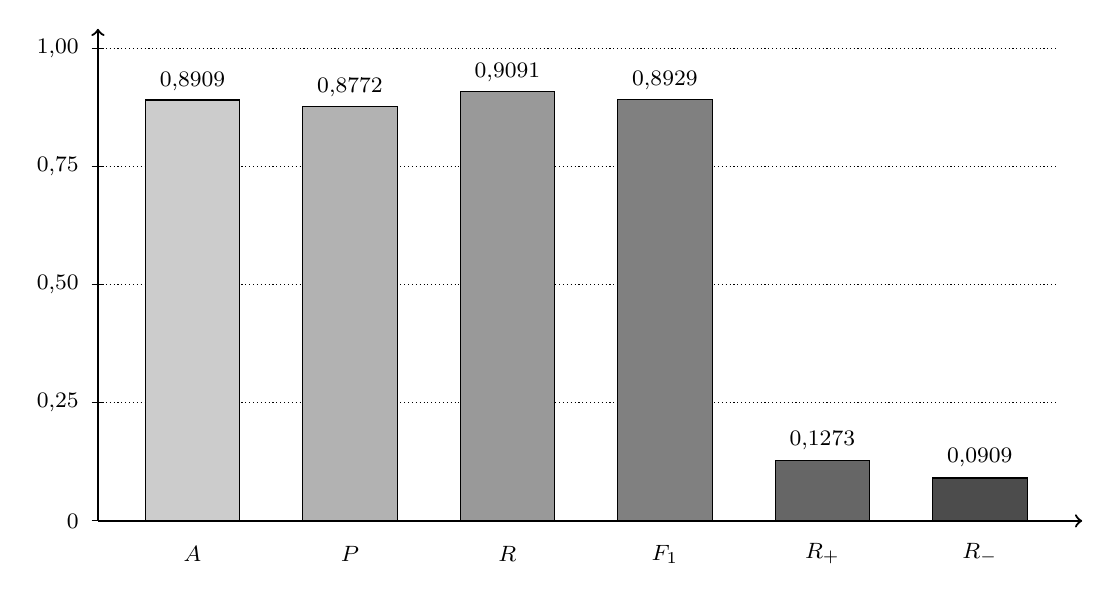
\begin{tikzpicture}[x=1cm,y=1cm]
  \draw[->,thick] (0,0) -- (0,6.25);
  \draw[->,thick] (0,0) -- (12.5,0);
  \foreach \y/\v in {0/0,1.5/0{,}25,3/0{,}50,4.5/0{,}75,6/1{,}00}{
    \draw (-0.08,\y) -- (0.08,\y);
    \node[anchor=east,font=\footnotesize] at (-0.12,\y) {\v};
    \draw[densely dotted] (0.1,\y) -- (12.2,\y);
  }
  \filldraw[fill=black!20,draw=black] (0.6,0) rectangle (1.8,5.3454);
  \filldraw[fill=black!30,draw=black] (2.6,0) rectangle (3.8,5.2632);
  \filldraw[fill=black!40,draw=black] (4.6,0) rectangle (5.8,5.4546);
  \filldraw[fill=black!50,draw=black] (6.6,0) rectangle (7.8,5.3574);
  \filldraw[fill=black!60,draw=black] (8.6,0) rectangle (9.8,0.7638);
  \filldraw[fill=black!70,draw=black] (10.6,0) rectangle (11.8,0.5454);

  \node[font=\footnotesize] at (1.2,5.58) {0,8909};
  \node[font=\footnotesize] at (3.2,5.50) {0,8772};
  \node[font=\footnotesize] at (5.2,5.69) {0,9091};
  \node[font=\footnotesize] at (7.2,5.59) {0,8929};
  \node[font=\footnotesize] at (9.2,1.02) {0,1273};
  \node[font=\footnotesize] at (11.2,0.80) {0,0909};

  \node[font=\footnotesize] at (1.2,-0.42) {$A$};
  \node[font=\footnotesize] at (3.2,-0.42) {$P$};
  \node[font=\footnotesize] at (5.2,-0.42) {$R$};
  \node[font=\footnotesize] at (7.2,-0.42) {$F_1$};
  \node[font=\footnotesize] at (9.2,-0.42) {$R_+$};
  \node[font=\footnotesize] at (11.2,-0.42) {$R_-$};
\end{tikzpicture}
\caption{Показники, арифметично одержані з агрегованої матриці помилок}
\label{fig:metric_comparison}
\end{figure}


Компонентне зіставлення попереднього прогону наведено в табл.~\ref{tab:ch4_component_results}. Перші чотири рядки характеризують окремі канали й спільну конфігурацію. Наступні три рядки відображають втручання в зафіксоване правило без повторного навчання. Їх не можна тлумачити як незалежне оцінювання нових скорочених моделей.

\begin{table}[htbp]
\caption{Агреговані результати окремих каналів і компонентного вилучення}
\label{tab:ch4_component_results}
\centering
\scriptsize
\resizebox{\textwidth}{!}{%
\begin{tabular}{lrrrrrrr}
\toprule
Конфігурація & Правильність & Точність & Повнота & $F_1$ & Хибнопозитивні & Хибнонегативні & Площа \\
\midrule
Структурний канал & 0,6364 & 0,6027 & 0,8000 & 0,6875 & 0,5273 & 0,2000 & 0,7914* \\
Спектрально-зоровий канал & 0,7273 & 1,0000 & 0,4545 & 0,6250 & 0,0000 & 0,5455 & 0,7569* \\
Скорочена правилова оцінка & 0,5000 & н/в** & 0,0000 & н/в** & 0,0000 & 1,0000 & 0,7273* \\
Спільна конфігурація & 0,8909 & 0,8772 & 0,9091 & 0,8929 & 0,1273 & 0,0909 & 0,9367* \\
\midrule
Без структурних ознак & 0,7545 & 1,0000 & 0,5091 & 0,6747 & 0,0000 & 0,4909 & 0,7473* \\
Без спектрально-зорових ознак & 0,7364 & 0,8611 & 0,5636 & 0,6813 & 0,0909 & 0,4364 & 0,7914* \\
Без скороченого правилового вектора & 0,8909 & 0,8772 & 0,9091 & 0,8929 & 0,1273 & 0,0909 & 0,9367* \\
\bottomrule
\end{tabular}}

\vspace{2pt}
\parbox{0.96\textwidth}{\footnotesize * Значення площі перенесено зі збереженого опису; без неперервних оцінок його повторно не обчислено. ** Скорочена правилова оцінка не сформувала жодного позитивного рішення, тому точність позитивного рішення й $F_1$ не визначені (ділення $0/0$); повнота при цьому дорівнює нулю коректно, оскільки жодного зі змінених об’єктів не виявлено.}
\end{table}

Після вилучення структурних ознак повнота зменшилася на $40{,}00$ відсоткового пункту, а після вилучення спектрально-зорових --- на $34{,}55$ відсоткового пункту. Отже, зафіксоване правило було чутливим до обох статичних входів. Однак нульова заміна, відсутність повторного навчання та використання того самого набору для налаштування й оцінювання не дають змоги встановити причинний внесок кожної групи або статистичну значущість різниці.

Вилучення скороченого правилового вектора не змінило жодного агрегованого показника. Цей результат стосується лише доступної правилової оцінки попереднього прогону. Він не підтверджує й не спростовує повний метод поведінкового узгодження ознак різного походження, оскільки причинно пов’язаних журналів $X_b$, повного представлення $Z_b$ та навченої процедури перехресного зіставлення не було.

Часові підсумки попереднього прогону наведено в табл.~\ref{tab:ch4_timing_results}. Сума середніх чотирьох операцій дорівнює $418{,}09$~мс. Спектрально-зорова операція становить $98{,}49$~\% цього часу, тому саме вона визначає часові витрати виміряної частини.

\begin{table}[htbp]
\caption{Агреговане зведення часу чотирьох операцій попереднього прогону}
\label{tab:ch4_timing_results}
\centering
\small
\resizebox{\textwidth}{!}{%
\begin{tabular}{lrrrr}
\toprule
Операція & Середнє, мс & Медіана, мс & 95-й процентиль, мс & Частка, \% \\
\midrule
Структурний аналіз & 5,82 & 4,71 & 15,68 & 1,39 \\
Спектрально-зоровий аналіз & 411,77 & 293,48 & 1511,46 & 98,49 \\
Скорочена правилова оцінка & 0,36 & 0,31 & 0,53 & 0,09 \\
Інтеграція ознак & 0,14 & 0,13 & 0,19 & 0,03 \\
\midrule
Виміряна частина оброблення\textsuperscript{а} & 418,09 & 298,58 & 1530,80 & 100,00 \\
\bottomrule
\end{tabular}}

\vspace{2pt}
\parbox{0.96\textwidth}{\footnotesize \textsuperscript{а} Медіану та 95-й процентиль рядка ``Виміряна частина оброблення'' узято зі збереженого зведення попереднього прогону, де їх обчислено за розподілом пооб’єктних сум. Вони не дорівнюють сумі відповідних квантилів окремих операцій, оскільки квантилі не адитивні; середні значення, навпаки, додаються точно: $5{,}82+411{,}77+0{,}36+0{,}14=418{,}09$.}
\end{table}

Зі середнього $418{,}09$~мс арифметично випливає $2{,}39$ послідовно опрацьованого об’єкта за секунду. Це значення не є пропускною здатністю розгорнутої веб-системи, оскільки не враховує приймання, чергу, прийняття рішення, реєстрацію, конкурентний доступ і передавання даних. Розподіл виміряного часу показано на рис.~\ref{fig:timing_breakdown}.

\begin{figure}[htbp]
\centering
\begin{tikzpicture}[x=0.13cm,y=1cm]
  \draw[fill=black!20,draw=black] (0,0) rectangle (1.39,1);
  \draw[fill=black!65,draw=black] (1.39,0) rectangle (99.88,1);
  \draw[fill=black!40,draw=black] (99.88,0) rectangle (99.97,1);
  \draw[fill=white,draw=black] (99.97,0) rectangle (100,1);
  \draw[thick] (0,0) rectangle (100,1);
  \node[white,font=\footnotesize] at (50.635,0.5)
    {аналіз спектральних і піксельних ознак: 98,49\%};
  \draw[->] (0.695,1.05) -- (8,2.1);
  \node[anchor=west,font=\footnotesize] at (8,2.1)
    {структурний аналіз: 1,39\%};
  \draw[->] (99.925,-0.05) -- (75,-1.05);
  \node[anchor=east,font=\footnotesize,align=right] at (75,-1.05)
    {оцінка ознак подій і поведінки за правилами: 0,09\%;\\інтеграція ознак: 0,03\%};
  \node[anchor=west,font=\footnotesize] at (0,-0.55) {0\%};
  \node[anchor=east,font=\footnotesize] at (100,-0.55) {100\%};
  \node[font=\footnotesize] at (50,-1.65)
    {прийняття рішення та реєстрацію результатів не враховано};
\end{tikzpicture}
\caption{Розподіл середнього часу між виміряними операціями}
\label{fig:timing_breakdown}
\end{figure}


Окреме категоріальне зведення попереднього опису дає зважене середнє $424{,}72$~мс, яке не збігається з операційним значенням $418{,}09$~мс. Без первинного часового журналу неможливо встановити, чи спричинена різниця складом груп, порядком усереднення або різними запусками. Тому категоріальне середнє не використано для висновку, а часові результати ретроспективного й внутрішнього циклів не зіставляються як показник прискорення.

У першій зовнішній серії середній виміряний час формування структурних і спектрально-зорових ознак для стандартизованого 12-кадрового фрагмента становив $830{,}268$~мс, а для повного первинного MP4 --- $18\,187{,}221$~мс. Ці значення не зіставляються як оцінка прискорення або уповільнення, оскільки фрагменти й повні записи відрізнялися тривалістю та просторовою роздільністю. Вони показують, що збільшення кількості декодованих кадрів безпосередньо збільшує вартість спектрально-зорового аналізу й має враховуватися під час вибору між синхронним опрацюванням та попередньою ізоляцією відеооб’єкта.

Загальна тривалість службових запусків не використовується як показник швидкодії. Вона залежала від повторного використання підготовлених об’єктів, кількості робочих потоків, перевірки контрольних сум і формування звітів. Для порівняння конфігурацій застосовано лише однопотокове ресурсне вимірювання на однаковій підмножині, наведене в табл.~\ref{tab:ch4_efficiency_results}.

Предметне тлумачення результатів визначається межами протоколу. Внутрішній цикл усунув змішування похідних спільного походження та зберіг пооб’єктні оцінки, однак його базові сцени були синтетичними, а види змін --- наперед відомими. Чотири зовнішні набори разом охопили $38$ природних записів із $12$ пристроїв, проте тисячі похідних залишаються залежними від малої кількості джерел. Ретроспективний цикл характеризує попередню конфігурацію, але не має незалежного поділу й повного первинного журналу. Основні межі систематизовано в табл.~\ref{tab:ch4_validity_limits}.

\begin{table}[htbp]
\caption{Межі тлумачення експериментальних результатів}
\label{tab:ch4_validity_limits}
\centering
\small
\begin{tabularx}{\textwidth}{p{0.24\textwidth}Y Y}
\toprule
Аспект & Установлена межа & Наслідок для висновку \\
\midrule
Походження даних & Внутрішній набір синтетичний; зовнішні набори містять $38$ природних записів із $12$ пристроїв; попередній набір не має повного реєстру & Оцінено перенесення на нові записи, але не встановлено універсальності для довільних пристроїв, сцен і способів кодування \\
Залежність спостережень & $56$, $32$, $10\,000$ і $2000$ похідних утворено відповідно з $8$, $4$, $4$ і $8$ груп ``пристрій--сцена'', тобто разом із $24$ зовнішніх груп походження; дві останні серії додатково поділено на $500$ і $100$ базових фрагментів. Загалом зовнішні набори охоплюють $38$ природних записів із $12$ пристроїв & Кількість похідних не можна прирівнювати до кількості незалежних джерел; повторне вибирання виконано за групами й вихідними записами, а умовні інтервали характеризують саме наявні записи \\
Предмет позитивної мітки & Мітка позначає контрольовану структурну або статистичну зміну & Не підтверджено виявлення або виконання аномального програмного коду \\
Охоплення форматів & PNG, JPEG, WebP, MP4 і WebM оцінено в багатоформатній та незалежній серіях; для JPEG, WebP і WebM виконано перенесення без повторного навчання & Підтверджено працездатність у заданих умовах, але не всі кодеки, профілі та реалізації форматів \\
Охоплення сценаріїв & Навчуваний шлюз не виявив жодної з $500$ суто спектральних змін незалежної серії & Висока специфічність і збалансований показник не доводять придатності до всіх видів прихованого впливу \\
Поведінкові дані & У $4832$ унікальних відеооб’єктах доступна технічна ознака не спрацювала; журнали $X_b$ і повне $Z_b$ не сформовано & Перевірено узгодження статичних оцінок, але не повний причинно-поведінковий метод і не повне представлення $Z$ \\
Ресурсне оцінювання & Час і пам’ять виміряно в п’яти однопотокових процесних запусках; апаратний паспорт, черга, паралельне навантаження й дії у відповідь відсутні & Значення придатні для внутрішнього порівняння реалізацій, але не визначають пропускної здатності розгорнутої веб-системи \\
Інтегральний показник & Редакцію $K_E$ сформовано після первинного перегляду якості, а ресурсну частину оцінено на підмножині даних розроблення & Рейтинг є розвідувальним; його потрібно підтвердити на нових джерелах і незалежному ресурсному запуску \\
\bottomrule
\end{tabularx}
\end{table}

Інтегральний показник $K_E$ не утворюється механічним об’єднанням результатів шести серій. Його обчислено лише для конфігурацій, які пройшли єдине багатоформатне й ресурсне оцінювання. Ретроспективне значення $0{,}8909$, внутрішнє значення $0{,}9750$ і результати незалежної підтверджувальної серії мають інші одиниці аналізу та не входять до одного бала. Завдяки цьому $K_E$ характеризує конкретний сценарій вибору, а не всю інформаційну технологію.

Послідовність серій змінила початковий висновок. У синтетичному наборі спільний опис $H$ усунув більшість помилок ізольованої спектрально-зорової конфігурації. Перша зовнішня серія не відтворила його переваги над структурною конфігурацією. Багатоформатна серія, зі свого боку, виявила межу вже структурної конфігурації на WebM і показала, що спільний опис має рівномірніший форматний профіль. Навчуваний шлюз усунув хибнопозитивні рішення на нових пристроях, але знизив повноту й не виявив суто спектральних змін. Отже, жодна конфігурація не є безумовно найкращою: структурна мінімізує ресурсні витрати, спільна зберігає більшу повноту, а шлюз надає перевагу специфічності.

Відсутність поведінкового спрацювання у $4832$ унікальних відеооб’єктах пояснює, чому результати навчуваного шлюзу визначалися статичними оцінками. Це не свідчить про нульову цінність причинно пов’язаних подій, яких у дослідженні не було. Для перевірки повного методу потрібні парні журнали штатного й зміненого оброблення того самого об’єкта, причинне пов’язування подій із фазами, навчання кодувальника лише на навчальній частині та одноразове оцінювання на нових групах.

Отже, експерименти підтвердили діагностичну придатність структурного аналізу для контрольованих контейнерних втручань, установили форматну межу його перенесення, кількісно описали компроміс між специфічністю, повнотою та ресурсними витратами й незалежно перевірили скорочений шлюз узгодження. Вони не підтверджують повний мультимодальний контур, виявлення виконуваного аномального коду або промислову готовність технології. Практичне застосування на цьому етапі має передбачати ізоляцію та експертну перевірку позитивного рішення, а не безумовне автоматичне блокування.

\section*{Висновки до розділу 4}
\addcontentsline{toc}{section}{Висновки до розділу 4}

\begin{enumerate}[label=\arabic*.]
\item Експериментальне дослідження охопило шість серій та окреме ресурсне вимірювання. Для внутрішньої серії сформовано $200$ первинних груп і $400$ PNG- та MP4-об’єктів із поділом $60:20:20$. Чотири зовнішні набори містили $38$ неповторюваних природних записів із $12$ пристроїв; багатоформатна серія охопила $10\,000$ похідних, а незалежна підтверджувальна --- $2000$. Кількість похідних не прирівнювалася до кількості незалежних джерел.

\item На внутрішній перевірній частині з $80$ об’єктів спільний статичний опис $H$ дав $40$ правильно визначених контрольних, жодного хибнопозитивного, два хибнонегативні та $38$ правильно визначених змінених об’єктів. Частка правильних рішень становила $0{,}9750$, повнота --- $0{,}9500$, $F_1=0{,}9744$, а площа під характеристичною кривою --- $0{,}9869$. Числова перевага над спектрально-зоровою конфігурацією була виразною, тоді як парна відмінність від структурної конфігурації не досягла рівня $0{,}05$ ($p=0{,}0625$). Тому внутрішня серія підтвердила корисність структурних ознак як доповнення до $Z_v$, але не довела загальної переваги $H$ над $Z_s$.

\item Перша зовнішня серія на $56$ похідних MP4 не відтворила внутрішньої переваги спільного опису над структурною конфігурацією. Для $Z_s$ збалансована частка правильних рішень становила $0{,}8333$, для $H$ --- $0{,}7857$, а для $Z_v$ --- $0{,}5000$. На цьому етапі саме структурне свідчення збереглося після переходу до природних MP4, тоді як перенесення роздільної здатності реалізованих спектрально-зорових ознак не підтверджено.

\item Багатоформатна серія показала, що структурна, спектрально-зорова та спільна конфігурації мають збалансовані частки правильних рішень $0{,}7636$, $0{,}5001$ і $0{,}7916$. Структурна конфігурація дала $0{,}5000$ на WebM, тоді як спільний опис мав форматні значення від $0{,}7387$ до $0{,}8173$. Отже, висновок першої MP4-серії не переноситься безумовно на всі формати. Класичні статистичні показники окремо залишилися поблизу $0{,}5$ і не забезпечили проходження форматного допуску після об’єднання зі структурним рішенням.

\item У незалежній серії навчуваний шлюз підвищив збалансовану частку правильних рішень від $0{,}7827$ до $0{,}8307$ й усунув $76$ хибнопозитивних рішень, але додав $84$ пропуски, зменшив загальну частку правильних рішень від $0{,}7500$ до $0{,}7460$ та не виявив жодної з $500$ суто спектральних змін. Критерій Мак-Немара дав $p=0{,}5801$. Отже, підтверджено профіль із пріоритетом специфічності, а не безумовну перевагу за всіма показниками.

\item Ресурсне вимірювання в п’яти процесних запусках дало 95-ті процентилі $2{,}136$, $760{,}662$, $853{,}971$ і $1078{,}904$~мс та значення пам’яті $78{,}77$, $96{,}79$, $101{,}53$ і $110{,}05$~МіБ відповідно для структурної, спектрально-зорової, спільної й навчуваної конфігурацій. Розвідувальний $K_E$ становив $77{,}50$, $50{,}69$, $68{,}95$ і $69{,}46$. Структурна конфігурація посіла перше місце завдяки швидкодії, але не пройшла форматного допуску; тому інтегральний бал тлумачиться лише разом із первинними складниками.

\item Ретроспективна перевірка $110$ об’єктів установила арифметичну узгодженість матриці $48$, $7$, $5$, $50$ та похідних від неї показників: правильності $0{,}8909$, точності позитивного рішення $0{,}8772$, повноти $0{,}9091$ і $F_1=0{,}8929$. Значення площі $0{,}9367$ без пооб’єктних оцінок не відтворено, а компонентне вилучення характеризує лише чутливість зафіксованого правила. Середній час $418{,}09$~мс стосується чотирьох операцій попередньої конфігурації; внутрішні $53{,}89$~мс для PNG і $198{,}76$~мс для MP4 та зовнішні $830{,}268$~мс для 12-кадрового фрагмента охоплюють лише формування статичних ознак.

\item Повну конфігурацію методу поведінкового узгодження експериментально не перевірено: причинно пов’язані журнали $X_b$ і повне представлення $Z_b$ не сформовано, а доступна технічна ознака не спрацювала у $4832$ унікальних відеооб’єктах. Позитивна мітка позначала контрольовану зміну, а не виконання аномального коду. Перенесення перевірено для п’яти форматів, але повний промисловий контур, паралельне навантаження та дії у відповідь залишаються поза межами одержаного підтвердження.
\end{enumerate}
